% Options for packages loaded elsewhere
% Options for packages loaded elsewhere
\PassOptionsToPackage{unicode}{hyperref}
\PassOptionsToPackage{hyphens}{url}
\PassOptionsToPackage{dvipsnames,svgnames,x11names}{xcolor}
%
\documentclass[
  number]{elsarticle}
\usepackage{xcolor}
\usepackage{amsmath,amssymb}
\setcounter{secnumdepth}{5}
\usepackage{iftex}
\ifPDFTeX
  \usepackage[T1]{fontenc}
  \usepackage[utf8]{inputenc}
  \usepackage{textcomp} % provide euro and other symbols
\else % if luatex or xetex
  \usepackage{unicode-math} % this also loads fontspec
  \defaultfontfeatures{Scale=MatchLowercase}
  \defaultfontfeatures[\rmfamily]{Ligatures=TeX,Scale=1}
\fi
\usepackage{lmodern}
\ifPDFTeX\else
  % xetex/luatex font selection
\fi
% Use upquote if available, for straight quotes in verbatim environments
\IfFileExists{upquote.sty}{\usepackage{upquote}}{}
\IfFileExists{microtype.sty}{% use microtype if available
  \usepackage[]{microtype}
  \UseMicrotypeSet[protrusion]{basicmath} % disable protrusion for tt fonts
}{}
\makeatletter
\@ifundefined{KOMAClassName}{% if non-KOMA class
  \IfFileExists{parskip.sty}{%
    \usepackage{parskip}
  }{% else
    \setlength{\parindent}{0pt}
    \setlength{\parskip}{6pt plus 2pt minus 1pt}}
}{% if KOMA class
  \KOMAoptions{parskip=half}}
\makeatother
% Make \paragraph and \subparagraph free-standing
\makeatletter
\ifx\paragraph\undefined\else
  \let\oldparagraph\paragraph
  \renewcommand{\paragraph}{
    \@ifstar
      \xxxParagraphStar
      \xxxParagraphNoStar
  }
  \newcommand{\xxxParagraphStar}[1]{\oldparagraph*{#1}\mbox{}}
  \newcommand{\xxxParagraphNoStar}[1]{\oldparagraph{#1}\mbox{}}
\fi
\ifx\subparagraph\undefined\else
  \let\oldsubparagraph\subparagraph
  \renewcommand{\subparagraph}{
    \@ifstar
      \xxxSubParagraphStar
      \xxxSubParagraphNoStar
  }
  \newcommand{\xxxSubParagraphStar}[1]{\oldsubparagraph*{#1}\mbox{}}
  \newcommand{\xxxSubParagraphNoStar}[1]{\oldsubparagraph{#1}\mbox{}}
\fi
\makeatother


\usepackage{longtable,booktabs,array}
\newcounter{none} % for unnumbered tables
\usepackage{calc} % for calculating minipage widths
% Correct order of tables after \paragraph or \subparagraph
\usepackage{etoolbox}
\makeatletter
\patchcmd\longtable{\par}{\if@noskipsec\mbox{}\fi\par}{}{}
\makeatother
% Allow footnotes in longtable head/foot
\IfFileExists{footnotehyper.sty}{\usepackage{footnotehyper}}{\usepackage{footnote}}
\makesavenoteenv{longtable}
\usepackage{graphicx}
\makeatletter
\newsavebox\pandoc@box
\newcommand*\pandocbounded[1]{% scales image to fit in text height/width
  \sbox\pandoc@box{#1}%
  \Gscale@div\@tempa{\textheight}{\dimexpr\ht\pandoc@box+\dp\pandoc@box\relax}%
  \Gscale@div\@tempb{\linewidth}{\wd\pandoc@box}%
  \ifdim\@tempb\p@<\@tempa\p@\let\@tempa\@tempb\fi% select the smaller of both
  \ifdim\@tempa\p@<\p@\scalebox{\@tempa}{\usebox\pandoc@box}%
  \else\usebox{\pandoc@box}%
  \fi%
}
% Set default figure placement to htbp
\def\fps@figure{htbp}
\makeatother





\setlength{\emergencystretch}{3em} % prevent overfull lines

\providecommand{\tightlist}{%
  \setlength{\itemsep}{0pt}\setlength{\parskip}{0pt}}



 
\usepackage[]{natbib}
\bibliographystyle{elsarticle-num}


\makeatletter
\@ifpackageloaded{caption}{}{\usepackage{caption}}
\AtBeginDocument{%
\ifdefined\contentsname
  \renewcommand*\contentsname{Table of contents}
\else
  \newcommand\contentsname{Table of contents}
\fi
\ifdefined\listfigurename
  \renewcommand*\listfigurename{List of Figures}
\else
  \newcommand\listfigurename{List of Figures}
\fi
\ifdefined\listtablename
  \renewcommand*\listtablename{List of Tables}
\else
  \newcommand\listtablename{List of Tables}
\fi
\ifdefined\figurename
  \renewcommand*\figurename{Figure}
\else
  \newcommand\figurename{Figure}
\fi
\ifdefined\tablename
  \renewcommand*\tablename{Table}
\else
  \newcommand\tablename{Table}
\fi
}
\@ifpackageloaded{float}{}{\usepackage{float}}
\floatstyle{ruled}
\@ifundefined{c@chapter}{\newfloat{codelisting}{h}{lop}}{\newfloat{codelisting}{h}{lop}[chapter]}
\floatname{codelisting}{Listing}
\newcommand*\listoflistings{\listof{codelisting}{List of Listings}}
\makeatother
\makeatletter
\makeatother
\makeatletter
\@ifpackageloaded{caption}{}{\usepackage{caption}}
\@ifpackageloaded{subcaption}{}{\usepackage{subcaption}}
\makeatother
\journal{Machine Learning with Applications}
\usepackage{bookmark}
\IfFileExists{xurl.sty}{\usepackage{xurl}}{} % add URL line breaks if available
\urlstyle{same}
% fallback for those not using the hyperref driver hyperxmp:
\makeatletter
\@ifundefined{xmpquote}{\newcommand{\xmpquote}[1]{#1}}{}
\makeatother
\hypersetup{
  pdftitle={A Reproducible Methodological Framework for Prosecutorial Congestion Risk Prediction Using Explainable Machine Learning and Temporal Validation},
  pdfauthor={Moisés Evangelista Gamarra; Jerremi Aron Chancan Labajos},
  pdfkeywords={\xmpquote{Machine learning}, \xmpquote{prosecutorial
analytics}, \xmpquote{judicial analytics}, \xmpquote{congestion
risk}, \xmpquote{explainable artificial intelligence}},
  colorlinks=true,
  linkcolor={blue},
  filecolor={Maroon},
  citecolor={Blue},
  urlcolor={Blue},
  pdfcreator={LaTeX via pandoc}}


\setlength{\parindent}{6pt}
\begin{document}

\begin{frontmatter}
\title{A Reproducible Methodological Framework for Prosecutorial
Congestion Risk Prediction Using Explainable Machine Learning and
Temporal Validation}
\author[1]{Moisés Evangelista Gamarra%
%
}
 \ead{mevangelistag@senati.pe} 
\author[1]{Jerremi Aron Chancan Labajos%
%
}
 \ead{152048@senati.pe} 

\affiliation[1]{organization={Servicio Nacional de Adiestramiento en
Trabajo Industrial
(SENATI)},city={Lima},country={Perú},countrysep={,},postcodesep={}}

\cortext[cor1]{Corresponding author}


        
\begin{abstract}
Congestion in justice systems poses a significant challenge for
institutional planning due to its impact on operational workload and
resource allocation. This study proposes a reproducible machine learning
framework to estimate the proxy risk of prosecutorial congestion using
administrative records from the Public Prosecutor\textquotesingle s
Office of Peru covering the 2019--2026 period. The methodology
integrates consensus-based robust feature selection, temporal validation
to prevent data leakage, robustness assessment, ablation analysis, and
SHAP-based interpretability within a single reproducible workflow. The
selected model achieved an F1-score of 0.469 and a ROC-AUC of 0.798 on
the 2025 test set while maintaining consistent performance during
external temporal validation on the 2026 dataset. The ablation study and
SHAP analysis indicate that the model\textquotesingle s predictive
capability is driven primarily by territorial and institutional
patterns, whereas historical features provide complementary information.
Furthermore, the operational impact analysis highlights the
model\textquotesingle s potential to support the preventive
prioritization of operational combinations with higher estimated proxy
risk. The main contribution of this work is a reproducible
methodological framework that integrates robust feature selection,
temporal validation, robustness assessment, and model interpretability
into a unified framework for supporting decision-making in the
prosecutorial domain.
\end{abstract}





\begin{keyword}
    Machine learning \sep prosecutorial analytics \sep judicial
analytics \sep congestion risk \sep 
    explainable artificial intelligence
\end{keyword}
\end{frontmatter}
    

\section{I. Introduction}\label{i.-introduction}

Congestion in justice systems represents a challenge for institutional
management, as it increases response times, hinders the efficient
allocation of resources, and limits the operational capacity of the
organizations responsible for the administration of justice. In this
context, machine learning has emerged as a promising tool for the early
identification of scenarios with high operational risk and for
supporting evidence-based planning through the analysis of
administrative records.

Several studies have applied machine learning techniques to predict
judicial congestion, workload, and institutional performance. However,
most studies evaluate predictive algorithms, feature selection
techniques, or interpretability methods in isolation, whereas aspects
such as temporal validation, explicit data leakage control, the
integration of robust feature selection and interpretability, and the
joint evaluation of model robustness remain uncommon within a single
reproducible methodological workflow.

In response to these limitations, this study proposes a reproducible
Consensus, Temporal Validation, and Explainability Methodological
Framework (CTVEMF) based on machine learning to estimate the proxy risk
of prosecutorial congestion in the Public Prosecutor\textquotesingle s
Office of Peru, using administrative records from the 2019--2026 period.
The main contributions of this work are as follows: (i) a
consensus-based robust feature selection strategy combining six methods,
preceded by an explicit multicollinearity audit; (ii) a year-block
temporal validation scheme that prevents data leakage; (iii) a joint
robustness assessment through an ablation study and unsupervised
validation of the feature space; and (iv) a SHAP-based interpretability
analysis integrated with an operational impact analysis aimed at the
preventive prioritization of operational combinations with higher
estimated risk. Collectively, these elements integrate, within a single
methodological workflow, components that the previous literature has
typically addressed in isolation.

The remainder of this paper is organized as follows. Section II presents
the related work. Section III describes the methodology. Section IV
presents the results. Sections V, VI, and VII present the discussion,
limitations, and conclusions, respectively.

\subsection{A. Machine Learning for Predicting Judicial and
Prosecutorial
Workload}\label{a.-machine-learning-for-predicting-judicial-and-prosecutorial-workload}

Previous research on predicting case duration and procedural delays has
predominantly focused on the judicial domain, overlooking prosecutorial
dynamics. Recent studies have shown that machine learning can contribute
to modeling operational workload and optimizing institutional
performance through the analysis of administrative records, including
applications aimed at reducing judicial congestion, evaluating
productivity, and conducting temporal analyses of judicial processes
\citep{azaria_alleviating_2024, vasconcelos_analysis_2023, pernici_improving_2024}.
While some studies combine tree-based models with explainability
techniques to improve the interpretation of predictions, others
incorporate process mining and temporal analysis to identify
bottlenecks, measure procedural duration, and evaluate institutional
performance using administrative data
\citep{azaria_alleviating_2024, pernici_improving_2024}. Although both
approaches have demonstrated promising results, each addresses only part
of the problem, and neither simultaneously integrates temporal
validation strategies, data leakage prevention, and robust feature
selection within a single methodological framework.

Although these studies demonstrate that administrative records can be
used to model operational congestion with promising results, their
methodological scope remains limited. In particular, they focus on
judicial scenarios following the prosecutorial investigation stage,
employ context-specific modeling strategies, and do not integrate
mechanisms to simultaneously address issues such as robust feature
selection, data leakage, and temporal validation. These limitations
restrict the reproducibility and generalizability of the models to
real-world operational scenarios. This evolution is also reflected in
recent review studies, which highlight a transition from isolated
predictive models toward comprehensive frameworks for the intelligent
management of judicial systems \citep{hannoon_artificial_2025}.

Overall, the literature indicates that the primary challenge no longer
lies solely in applying predictive algorithms to the judicial domain,
but rather in integrating robust feature selection, explicit data
leakage prevention, temporal validation, and explainability within a
single methodological framework to ensure reproducible and transferable
models for real-world operational scenarios. In this context, the
present study proposes a framework that integrates these components in a
unified manner within the prosecutorial domain.

\subsection{B. Feature Selection: Filter, Wrapper, Embedded, and
Ensemble
Approaches}\label{b.-feature-selection-filter-wrapper-embedded-and-ensemble-approaches}

Among the most relevant methodological components for building robust
predictive models, feature selection has assumed a central role due to
its impact on the stability, interpretability, and generalization
capability of classifiers. In contrast, wrapper methods explore these
interactions using the predictive performance of the classifier, but
they require greater computational cost \citep{zhou_efficient_2024}.
Embedded methods balance both aspects by incorporating feature selection
during model training; however, their performance continues to depend on
the algorithm employed. These differences have motivated the development
of consensus-based feature selection strategies that seek to combine the
strengths of multiple approaches and reduce the variability of the final
feature subset \citep{moslemi_tutorial-based_2023}. In turn,
all-relevant embedded feature selectors, such as the Boruta algorithm,
compare the importance of each feature against randomized copies (shadow
features) using a Random Forest, providing a statistically supported
relevance test rather than a minimum-optimal feature subset
\citep{kursa_feature_2010}.

Because individual feature selectors often produce different results in
the presence of highly correlated variables, their isolated use may
generate unstable feature subsets that depend on the selected algorithm.
Consequently, ensemble feature selection has emerged as an alternative
for increasing the robustness and stability of the process through the
aggregation of multiple selection criteria \citep{zhou_efficient_2024}.

From this perspective, the proposed framework implements a consensus
based on six complementary methods---two filter methods (MI and ANOVA),
one filter method for categorical variables (χ²), one embedded method
(Random Forest), and two wrapper methods (Boruta and RFECV)---with the
aim of combining methodological strengths and reducing dependence on a
single feature selection algorithm. This process is preceded by an
explicit multicollinearity audit using the Pearson correlation
coefficient and Cramér\textquotesingle s V coefficient.

Although several studies have proposed individual feature selection
strategies, the literature still reports limited integration between
feature space quality auditing, consensus-based feature selection, and
evaluation using explainable models within a reproducible methodological
workflow. The strategy adopted in this work responds precisely to this
need by integrating complementary approaches into a single robust
feature selection stage.

\subsection{C. Class Imbalance, Data Leakage, and Temporal
Validation}\label{c.-class-imbalance-data-leakage-and-temporal-validation}

Risk classification tasks based on administrative datasets often exhibit
substantial class imbalance, which motivates the use of resampling
techniques such as SMOTE, which generates synthetic instances of the
minority class through linear interpolation in the feature space
\citep{chawla_smote_2002}. The proposed framework avoids synthetic
resampling, instead adopting class weighting for compatible models
(Section III.D.2), since the observed class imbalance (86\%/14\%) did
not require an artificial expansion of the sample space. Nevertheless, a
critical and frequently overlooked concern in this domain is data
leakage; indeed, systematic reviews have confirmed that this
methodological flaw compromises the validity of hundreds of machine
learning studies across multiple disciplines, commonly induced by
computing preprocessing statistics on the entire dataset before data
partitioning \citep{kapoor_leakage_2023}.

Temporal validation and restricting preprocessing exclusively to the
training set are widely recommended to prevent information leakage and
ensure reproducible evaluation
\citep{kapoor_leakage_2023, sasse_leakage_2023}; omitting these
practices may lead to overly optimistic performance estimates and limit
the reproducibility of the results \citep{hamdan_julearn_2023}. In
response, recent studies have proposed leakage-free evaluation protocols
as a standard practice \citep{hamdan_julearn_2023}, an approach that
this framework adopts rigorously by computing all preprocessing
parameters exclusively on the training partition (Section III.B.1).

\subsection{D. Explainability and Responsible AI for Risk Prediction in
Judicial
Contexts}\label{d.-explainability-and-responsible-ai-for-risk-prediction-in-judicial-contexts}

Recent literature agrees that interpretability is an indispensable
requirement for the adoption of predictive models in judicial contexts
\citep{richmond_explainable_2024}; however, existing approaches differ
in their objectives, particularly in legal applications where
explanations must be understandable to different institutional
stakeholders \citep{richmond_explainable_2024}.

While tools such as SHAP aim to explain the internal behavior of complex
models through local and global feature attributions, consistent with
recent systematic reviews on Explainable AI \citep{saarela_recent_2024},
these perspectives should be understood as complementary rather than
mutually exclusive alternatives
\citep{lundberg_unified_2017, bhatnagar_hybrid_2025}. In parallel, risk
assessment tools in the criminal justice sector have been subject to
intense scrutiny; the literature reports that commercial algorithms
based on more than 100 variables did not outperform either in accuracy
or fairness the predictions made by individuals without legal expertise
\citep{dressel_accuracy_2018}. This evidence demonstrates that high
predictive accuracy alone is insufficient to support decision-making in
judicial contexts. Institutional trust also requires transparent,
interpretable, and auditable models capable of justifying their
predictions and facilitating their review by domain experts, in
accordance with the recent Responsible AI literature
\citep{taylor_is_2025}.

From this perspective, the proposed framework incorporates local
explanations through SHAP values and probabilistic calibration
diagnostics to promote the responsible use of predictions prior to any
potential institutional deployment. Consequently, the current challenge
extends beyond the isolated use of explainability techniques and
consists of incorporating them into comprehensive frameworks that
integrate rigorous validation, transparency, and reproducibility from
the methodological design stage.

Overall, the literature demonstrates significant advances in the
application of machine learning to the judicial domain, feature
selection, data leakage prevention, and model interpretability. However,
these components are typically addressed in isolation, with limited
integration into reproducible methodological frameworks that
simultaneously incorporate temporal validation, robust feature
selection, explainability, and evaluation tailored to the operational
context.

This methodological need motivates the proposal presented in the
following section, whose primary contribution is to integrate, within a
single reproducible framework, robust feature selection, data leakage
prevention, temporal validation, supervised learning, and
interpretability for the early identification of proxy signals of
prosecutorial congestion.

\section{III. Materials And Methods}\label{iii.-materials-and-methods}

\subsection{A. Dataset}\label{a.-dataset}

\subsubsection{1) Description}\label{description}

This study uses the administrative records from the "MPFN Fiscal Cases"
dataset, published by the Public Prosecutor\textquotesingle s Office --
Office of the Attorney General of Peru (MPFN) on the National Open Data
Platform
\citep{ministerio_publico__fiscalia_de_la_nacion_mpfn_mpfn_2022}. The
dataset reports the volume of cases received and processed nationwide,
disaggregated by prosecutorial district, prosecution office type,
subject matter, and specialty, and distributed in independent annual CSV
files covering the 2019--2026 period.

\subsubsection{2) Variables}\label{variables}

The official MPFN data dictionary comprises 16 raw administrative fields
structured into four dimensions: temporality, institutional geography,
case taxonomy, and volumetric workload, as described in Table I.

\textbf{TABLE I.} RAW ADMINISTRATIVE FIELDS FROM THE MPFN DATA
DICTIONARY

{\def\LTcaptype{none} % do not increment counter
\begin{longtable}[]{@{}
  >{\raggedright\arraybackslash}p{(\linewidth - 2\tabcolsep) * \real{0.2766}}
  >{\raggedright\arraybackslash}p{(\linewidth - 2\tabcolsep) * \real{0.7021}}@{}}
\toprule\noalign{}
\begin{minipage}[b]{\linewidth}\raggedright
\textbf{Dimension}
\end{minipage} & \begin{minipage}[b]{\linewidth}\raggedright
\textbf{Variables}
\end{minipage} \\
\midrule\noalign{}
\endhead
\bottomrule\noalign{}
\endlastfoot
Temporality & periodo, anio, fecha\_descarga, fecha\_corte \\
Institutional Geography & distrito\_fiscal, ubigeo\_pjfs*, dpto\_pjfs,
prov\_pjfs, dist\_pjfs \\
Case Taxonomy & tipo\_fiscalia, materia, especialidad, tipo\_caso,
especializada \\
Volumetric Workload & ingresado, atendido \\
\end{longtable}
}

Note: ubigeo\_pjfs is encoded according to the INEI catalog.

Based on these fields, 14 variables were constructed through feature
engineering and grouped into four families: operational pressure
indicators, temporal descriptors, second-order categorical interactions,
and lagged historical metrics by prosecutorial district, computed as
moving averages and year-over-year growth rates of case inflows and
processed cases from the previous period (Table II).

\textbf{TABLE II.} VARIABLES DERIVED THROUGH FEATURE ENGINEERING

{\def\LTcaptype{none} % do not increment counter
\begin{longtable}[]{@{}
  >{\raggedright\arraybackslash}p{(\linewidth - 2\tabcolsep) * \real{0.2467}}
  >{\raggedright\arraybackslash}p{(\linewidth - 2\tabcolsep) * \real{0.7445}}@{}}
\toprule\noalign{}
\begin{minipage}[b]{\linewidth}\raggedright
\textbf{Dimension}
\end{minipage} & \begin{minipage}[b]{\linewidth}\raggedright
\textbf{Variables}
\end{minipage} \\
\midrule\noalign{}
\endhead
\bottomrule\noalign{}
\endlastfoot
Operational Pressure & saldo\_casos, tasa\_atencion, ratio\_saldo \\
Temporal Descriptors & anio\_centrado†, post\_pandemia,
periodo\_pandemia\_2020 \\
Categorical Interactions (2nd Order) & inter\_distrito\_tipo\_caso,
inter\_materia\_tipo\_fiscalia, inter\_tipo\_fiscalia\_especialidad \\
Lagged Historical Metrics (by Prosecutorial District) &
hist\_ingresado\_mean\_prev\_dist\_pjfs,
hist\_atendido\_mean\_prev\_dist\_pjfs,
hist\_saldo\_mean\_prev\_dist\_pjfs,
growth\_ingresado\_prev\_dist\_pjfs,
growth\_atendido\_prev\_dist\_pjfs \\
\end{longtable}
}

Note: † Subsequently excluded from the candidate feature matrix due to
direct collinearity with the calendar year (Section III.B.5).

\subsubsection{3) Study Period}\label{study-period}

The unified dataset covers the period from January 2019 to May 2026
(partial), consolidating a matrix of 9,593 records after the integration
process. To simulate a real-world environment and eliminate any risk of
data leakage, the data partitioning was structured using a year-block
walk-forward cross-validation scheme (4 folds).

The chronological distribution was configured as follows: the 2019--2023
period was reserved for the primary training stage (subdivided into an
internal training block spanning 2019--2022 and an internal validation
block corresponding to 2023, used exclusively for consensus-based
feature selection); the 2024 block was allocated to the external
validation and probabilistic calibration stage; the 2025 observations
were isolated as the hold-out test set; finally, the available records
from 2026 were used as an independent prospective evaluation set. A
summary of these characteristics is presented in Table III.

\textbf{TABLE III.} GENERAL CHARACTERISTICS OF THE DATASET

{\def\LTcaptype{none} % do not increment counter
\begin{longtable}[]{@{}
  >{\raggedright\arraybackslash}p{(\linewidth - 2\tabcolsep) * \real{0.5405}}
  >{\raggedright\arraybackslash}p{(\linewidth - 2\tabcolsep) * \real{0.4324}}@{}}
\toprule\noalign{}
\begin{minipage}[b]{\linewidth}\raggedright
\textbf{Characteristic}
\end{minipage} & \begin{minipage}[b]{\linewidth}\raggedright
\textbf{Value}
\end{minipage} \\
\midrule\noalign{}
\endhead
\bottomrule\noalign{}
\endlastfoot
Source & MPFN -- Peru Open Data
\citep{ministerio_publico__fiscalia_de_la_nacion_mpfn_mpfn_2022} \\
Period & Jan.~2019 -- May 2026 \\
Total Records & 9,593 \\
Original Fields & 16 \\
Candidate Features (Initial) & 28 \\
After Pearson Filter (\textgreater0.90) & 26 \\
After Cramér\textquotesingle s V Filter (\textgreater0.80) & 17 \\
After Encoding (One-Hot + Frequency) & 433 \\
Final Features (6-Method Consensus) & 69 \\
Train/Valid/Test/External Split & 6076 / 1195 / 1199 / 1123 \\
Class Balance (Train) & 86.0\% / 14.0\% \\
Validation & Year-block, 4 folds \\
\end{longtable}
}

Note: The partition is reported as train/validation/test/external. Class
balance is expressed as Class 0 / Class 1.

\subsection{B. Methodological
Framework}\label{b.-methodological-framework}

The proposed framework consists of six sequential phases designed to
ensure the reproducibility, auditability, and temporal validity of the
system (Figure 1).

\pandocbounded{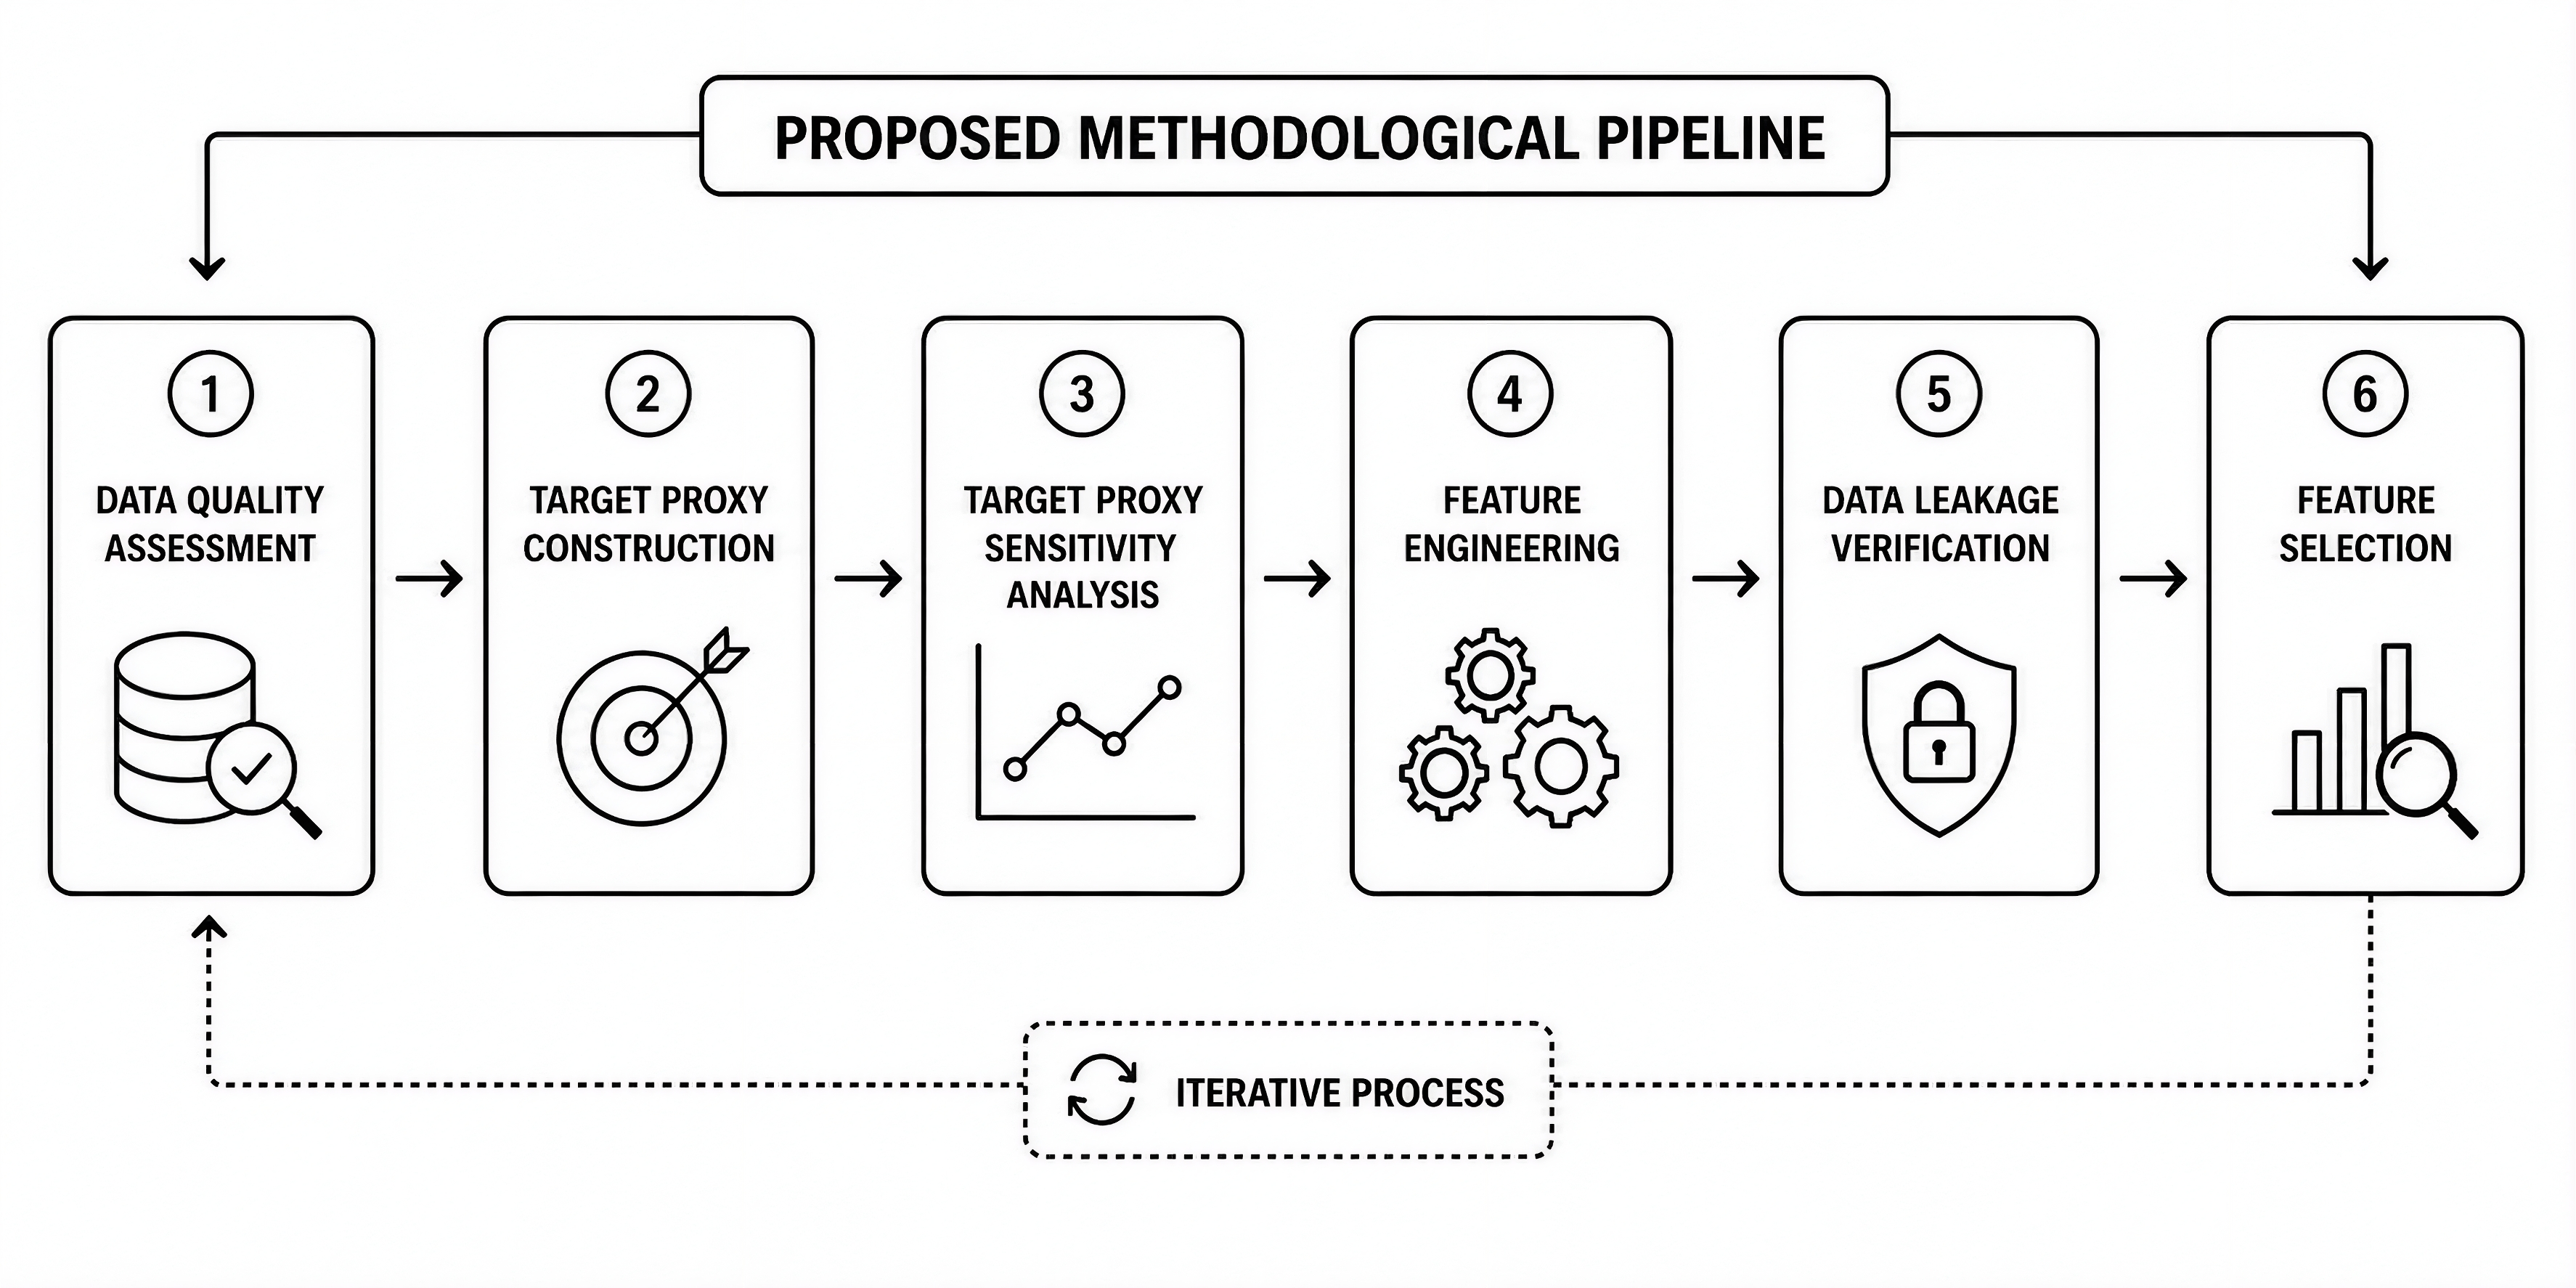
\includegraphics[keepaspectratio]{./media/image1.png}}

\textbf{Figure 1.} Methodological Framework of Consensus, Temporal
Validation, and Explainability for Fiscal Congestion

\subsubsection{1) Data Quality}\label{data-quality}

This phase included the normalization of categorical variables through
the removal of leading and trailing whitespace, standardization to
uppercase, and harmonization of missing values, as well as the detection
of redundant columns resulting from the annual data integration process
and the removal of duplicate records.

For the missing values identified in the \emph{ingresado} and
\emph{atendido} fields, imputation was performed using the median
computed exclusively from the temporal training blocks to mitigate data
leakage. In parallel, binary indicator variables (\emph{flag\_nulo\_})
were generated to preserve the missingness signal as a potentially
predictive attribute.

For categorical variables, missing values were imputed using an explicit
category (\emph{NO\_ESPECIFICADO}) instead of the mode, thereby avoiding
the introduction of an artificially dominant class. Finally, the
interquartile range (IQR) criterion was applied for the preliminary
profiling and identification of numerical outliers.

\subsubsection{2) Proxy Target}\label{proxy-target}

Let sᵢ = ingresadoᵢ − atendidoᵢ denote the case backlog and tᵢ =
atendidoᵢ / ingresadoᵢ the case processing rate for record \emph{i}. The
binary target variable \emph{riesgo\_congestion} is defined, under the
baseline scenario (P75/P25), as shown in Equation (1).

\[y_i = \mathbb{1}\left[s_i \geq q_{.75}(s_{\text{train}}) \wedge t_i \leq q_{.25}(t_{\text{train}})\right] \tag{1}\]

where the percentile thresholds \emph{q}\textsubscript{75} and
\emph{q}\textsubscript{25} are computed exclusively from the training
block. The framework formally defines this label as an operational proxy
signal rather than as an official certification of prosecutorial
congestion or a causal inference. This design follows a conservative
criterion aimed at isolating situations of severe operational overload
in an auditable manner.

\subsubsection{3) Target Sensitivity
Analysis}\label{target-sensitivity-analysis}

Since \emph{riesgo\_congestion} is a proxy label, its robustness to the
arbitrary selection of percentile thresholds must be verified before it
is adopted as the basis for modeling.

To this end, three alternative scenarios were established as a parallel
sensitivity analysis (Table IV).

\textbf{TABLE IV.} SENSITIVITY ANALYSIS OF THE PROXY TARGET ACROSS
SCENARIOS

{\def\LTcaptype{none} % do not increment counter
\begin{longtable}[]{@{}
  >{\raggedright\arraybackslash}p{(\linewidth - 10\tabcolsep) * \real{0.1818}}
  >{\raggedright\arraybackslash}p{(\linewidth - 10\tabcolsep) * \real{0.1591}}
  >{\raggedright\arraybackslash}p{(\linewidth - 10\tabcolsep) * \real{0.1477}}
  >{\raggedright\arraybackslash}p{(\linewidth - 10\tabcolsep) * \real{0.1364}}
  >{\raggedright\arraybackslash}p{(\linewidth - 10\tabcolsep) * \real{0.1705}}
  >{\raggedright\arraybackslash}p{(\linewidth - 10\tabcolsep) * \real{0.1818}}@{}}
\toprule\noalign{}
\endhead
\bottomrule\noalign{}
\endlastfoot
\textbf{Threshold} & \textbf{Train \%} & \textbf{Test \%} & \textbf{Ext
\%} & \textbf{CV} & \textbf{Role} \\
\textbf{P70/P30} & 19.4 & 19.8 & 26.3 & 0.165 (min.) & Early warning \\
\textbf{P75/P25} & 14.0 & 14.4 & 20.2 & 0.219 & Primary \\
\textbf{P80/P20} & 9.3 & 9.0 & 14.3 & 0.278 & Strict \\
\textbf{P85/P15} & 5.3 & 5.0 & 9.3 & 0.379 (max.) & Very strict \\
\end{longtable}
}

Note: Train \% = prevalence in the training set; Test \% = prevalence in
the 2025 test set; Ext \% = prevalence in the 2026 external dataset; CV
= interannual coefficient of variation (2019--2026); Role = operational
interpretation of the scenario.

The prevalence of Class 1 in the training set ranges from 5.3\%
(P85/P15) to 19.4\% (P70/P30), while the temporal stability of the event
rate---measured as the coefficient of variation (CV) between 2019 and
2026---increases monotonically with threshold severity (CV = 0.165 for
P70/P30 up to 0.379 for P85/P15). The baseline scenario (P75/P25, CV =
0.219, training prevalence = 14.0\%) is not the most stable among the
four scenarios---P70/P30 is---but it was retained because it provides
the best balance between institutional severity and sufficient class
balance for model training without resorting to synthetic resampling,
compared with the greater rarity and interannual variability of the
P80/P20 and P85/P15 scenarios.

\subsubsection{4) Feature Engineering}\label{feature-engineering}

The 14 derived variables were designed according to four criteria:
operational pressure indicators (imbalance between case inflows and
processed cases), pandemic-related temporal descriptors
(\emph{post\_pandemia}, \emph{periodo\_pandemia\_2020}), second-order
categorical interactions that capture nonlinear institutional synergies,
and lagged historical variables by prosecutorial district that
incorporate previous moving averages and growth rates without
introducing predictive anachronisms.

\subsubsection{5) Data Leakage Control}\label{data-leakage-control}

Because the target variable (\emph{riesgo\_congestion}) is constructed
directly from \emph{ingresado} and \emph{atendido}, these
attributes---\emph{ingresado}, \emph{atendido}, and their derived
variables \emph{saldo\_casos}, \emph{tasa\_atencion}, and
\emph{ratio\_saldo} (\emph{LEAKAGE\_COLS})---were isolated through a
strict exclusion list, together with non-predictive metadata and the
columns corresponding to the four alternative proxy scenarios.
Additionally, \emph{anio\_centrado} was excluded from the candidate
feature matrix because of its direct collinearity with the calendar year
(\emph{COLLINEAR\_EXCLUDE}).

\subsubsection{6) Feature Selection}\label{feature-selection}

A potential multicollinearity analysis was performed using the Pearson
correlation coefficient (r \textgreater{} 0.90) for numerical variables
and Cramér\textquotesingle s V (\textgreater{} 0.80) for categorical
variables (Figures 2--3).

\pandocbounded{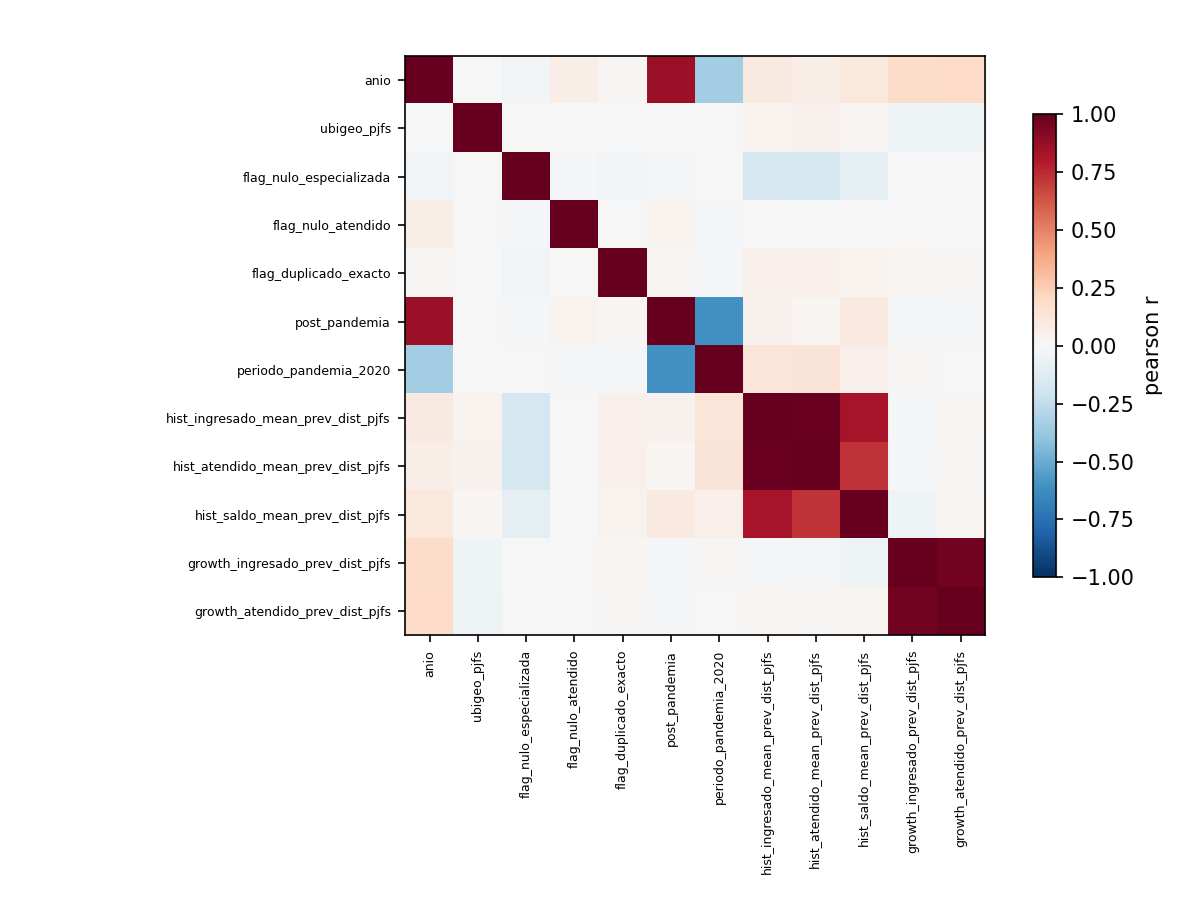
\includegraphics[keepaspectratio]{./media/image2.png}}

\textbf{Figure 2.} Pearson correlation among numerical variables.

\pandocbounded{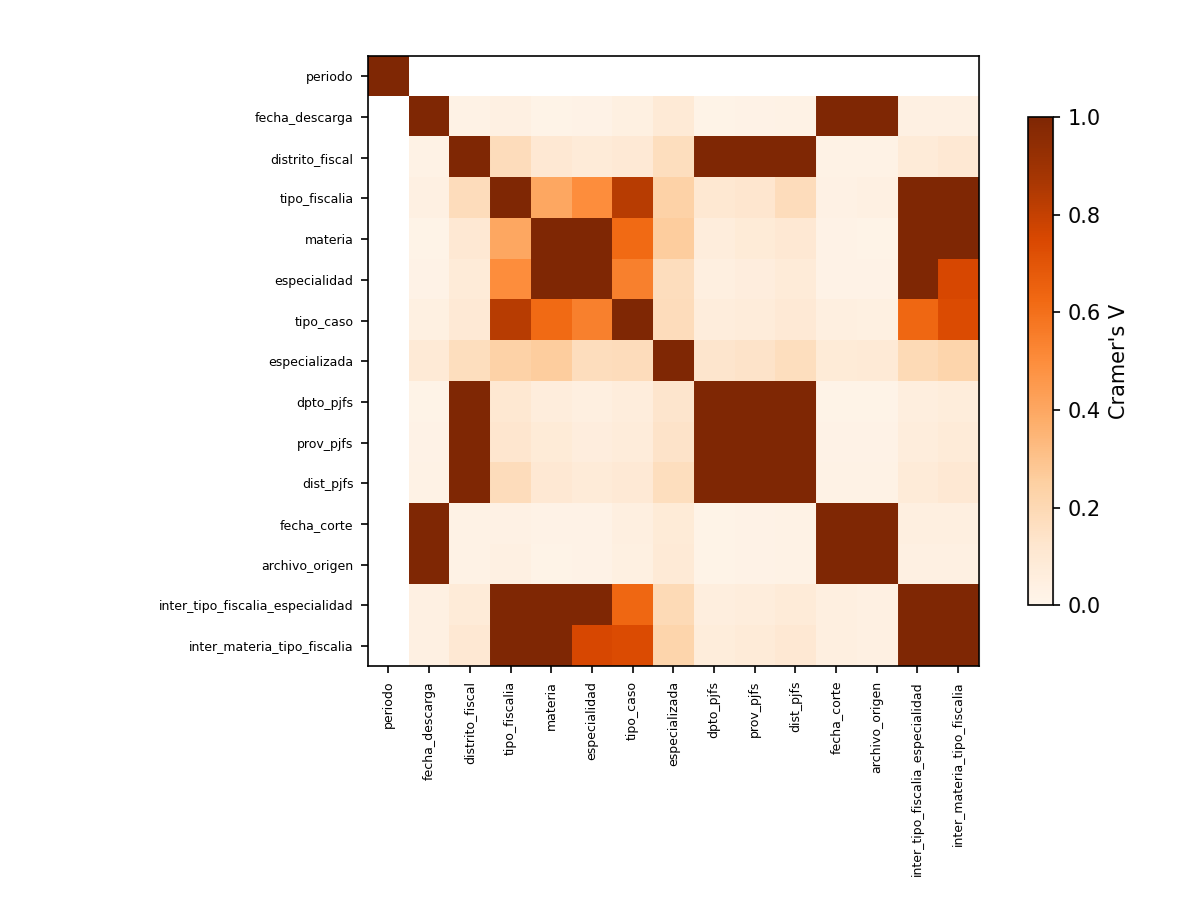
\includegraphics[keepaspectratio]{./media/image3.png}}

\textbf{Figure 3.} Cramér\textquotesingle s V correlation among
categorical variables.

Subsequently, six complementary feature selection methods---two
continuous filter methods, one categorical filter method, one embedded
method, and two wrapper methods (Table V)---were implemented, each
operating under the same year-block temporal cross-validation scheme.

\textbf{TABLE V.} FEATURE SELECTION METHODS EVALUATED

{\def\LTcaptype{none} % do not increment counter
\begin{longtable}[]{@{}
  >{\raggedright\arraybackslash}p{(\linewidth - 4\tabcolsep) * \real{0.2857}}
  >{\raggedright\arraybackslash}p{(\linewidth - 4\tabcolsep) * \real{0.4935}}
  >{\raggedright\arraybackslash}p{(\linewidth - 4\tabcolsep) * \real{0.1948}}@{}}
\toprule\noalign{}
\begin{minipage}[b]{\linewidth}\raggedright
\textbf{Method}
\end{minipage} & \begin{minipage}[b]{\linewidth}\raggedright
\textbf{Type}
\end{minipage} & \begin{minipage}[b]{\linewidth}\raggedright
\textbf{No.~vars}
\end{minipage} \\
\midrule\noalign{}
\endhead
\bottomrule\noalign{}
\endlastfoot
Mutual Information & Filter (Continuous) & 40 \\
ANOVA F-test & Filter (Continuous) & 40 \\
χ² & Filter (Categorical) & 40 \\
Random Forest & Embedded & 40 \\
Boruta & Wrapper (All-Relevant) & 12 \\
RFECV & Wrapper (Recursive + Temporal CV) & 52 \\
\end{longtable}
}

The consensus among methods is formalized by Equation (2), where each
term represents the binary vote of the corresponding method (1 if
feature \emph{i} is selected, 0 otherwise).

\[FeatureScore_i = \frac{MI_i + ANOVA_i + \chi^2_i + RF_i + Boruta_i + RFECV_i}{6} \tag{2}\]

The final features were determined using a consensus voting mechanism
with a minimum threshold of 2 out of 6 methods, resulting in a subset of
69 final features (Table VI).

\textbf{TABLE VI.} CONSENSUS VOTING DISTRIBUTION AND RETAINED FEATURES

{\def\LTcaptype{none} % do not increment counter
\begin{longtable}[]{@{}
  >{\raggedright\arraybackslash}p{(\linewidth - 4\tabcolsep) * \real{0.4933}}
  >{\raggedright\arraybackslash}p{(\linewidth - 4\tabcolsep) * \real{0.2000}}
  >{\raggedright\arraybackslash}p{(\linewidth - 4\tabcolsep) * \real{0.2800}}@{}}
\toprule\noalign{}
\begin{minipage}[b]{\linewidth}\raggedright
\textbf{Votes (6 methods)}
\end{minipage} & \begin{minipage}[b]{\linewidth}\raggedright
\textbf{No.~vars}
\end{minipage} & \begin{minipage}[b]{\linewidth}\raggedright
\textbf{\% Total (433)}
\end{minipage} \\
\midrule\noalign{}
\endhead
\bottomrule\noalign{}
\endlastfoot
6/6 (Unanimous) & 3 & 0.7\% \\
5/6 & 5 & 1.2\% \\
4/6 & 12 & 2.8\% \\
3/6 & 20 & 4.6\% \\
2/6 (Minimum Threshold) & 29 & 6.7\% \\
Retained Subtotal (≥2 Votes) & 69 & 15.9\% \\
1/6 (Discarded) & 15 & 3.5\% \\
0/6 (Discarded) & 349 & 80.6\% \\
\end{longtable}
}

Note: Consensus threshold = votes ≥ 2/6. The three features with
unanimous agreement (6/6) are freq\_distrito\_fiscal, freq\_tipo\_caso,
and tipo\_caso\_DENUNCIA.

\subsection{C. Feature Space
Validation}\label{c.-feature-space-validation}

The purpose was to examine the internal topology of the feature space
and evaluate the consistency of the proxy risk signal with the
multivariate structure of the data. The exploratory analyses (PCA,
t-SNE, and UMAP; Figures 4--6) confirmed the existence of nonlinear
structures with local clusters and partial overlap between classes,
thereby justifying the use of robust classifiers.

\pandocbounded{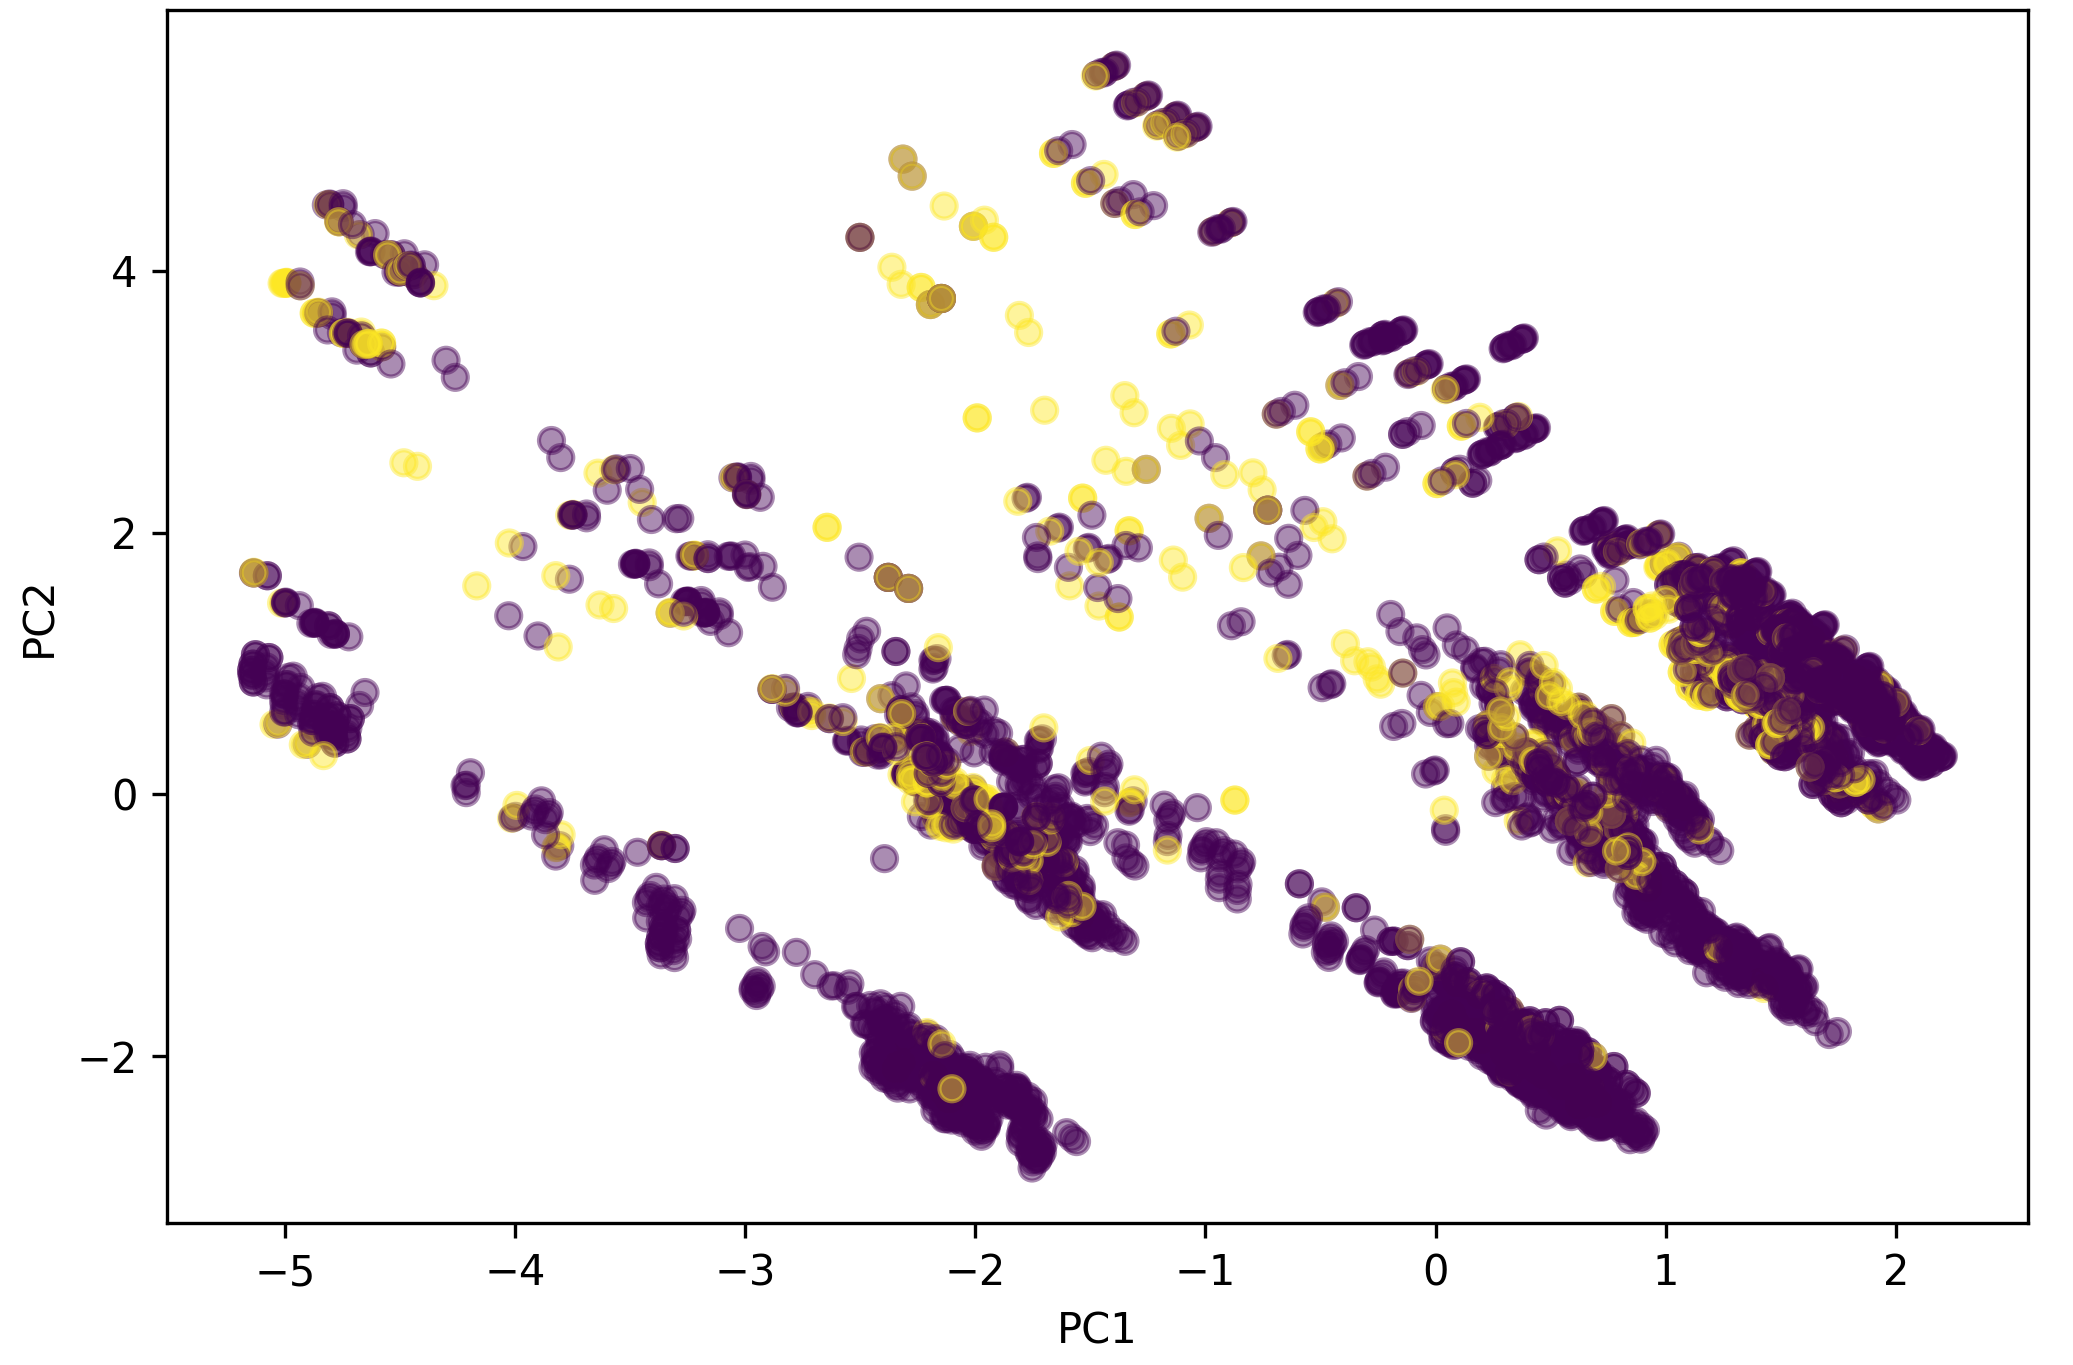
\includegraphics[keepaspectratio]{./media/image4.png}}

\textbf{Figure 4.} Two-dimensional PCA projection of the training set
colored according to the proxy target class.

\pandocbounded{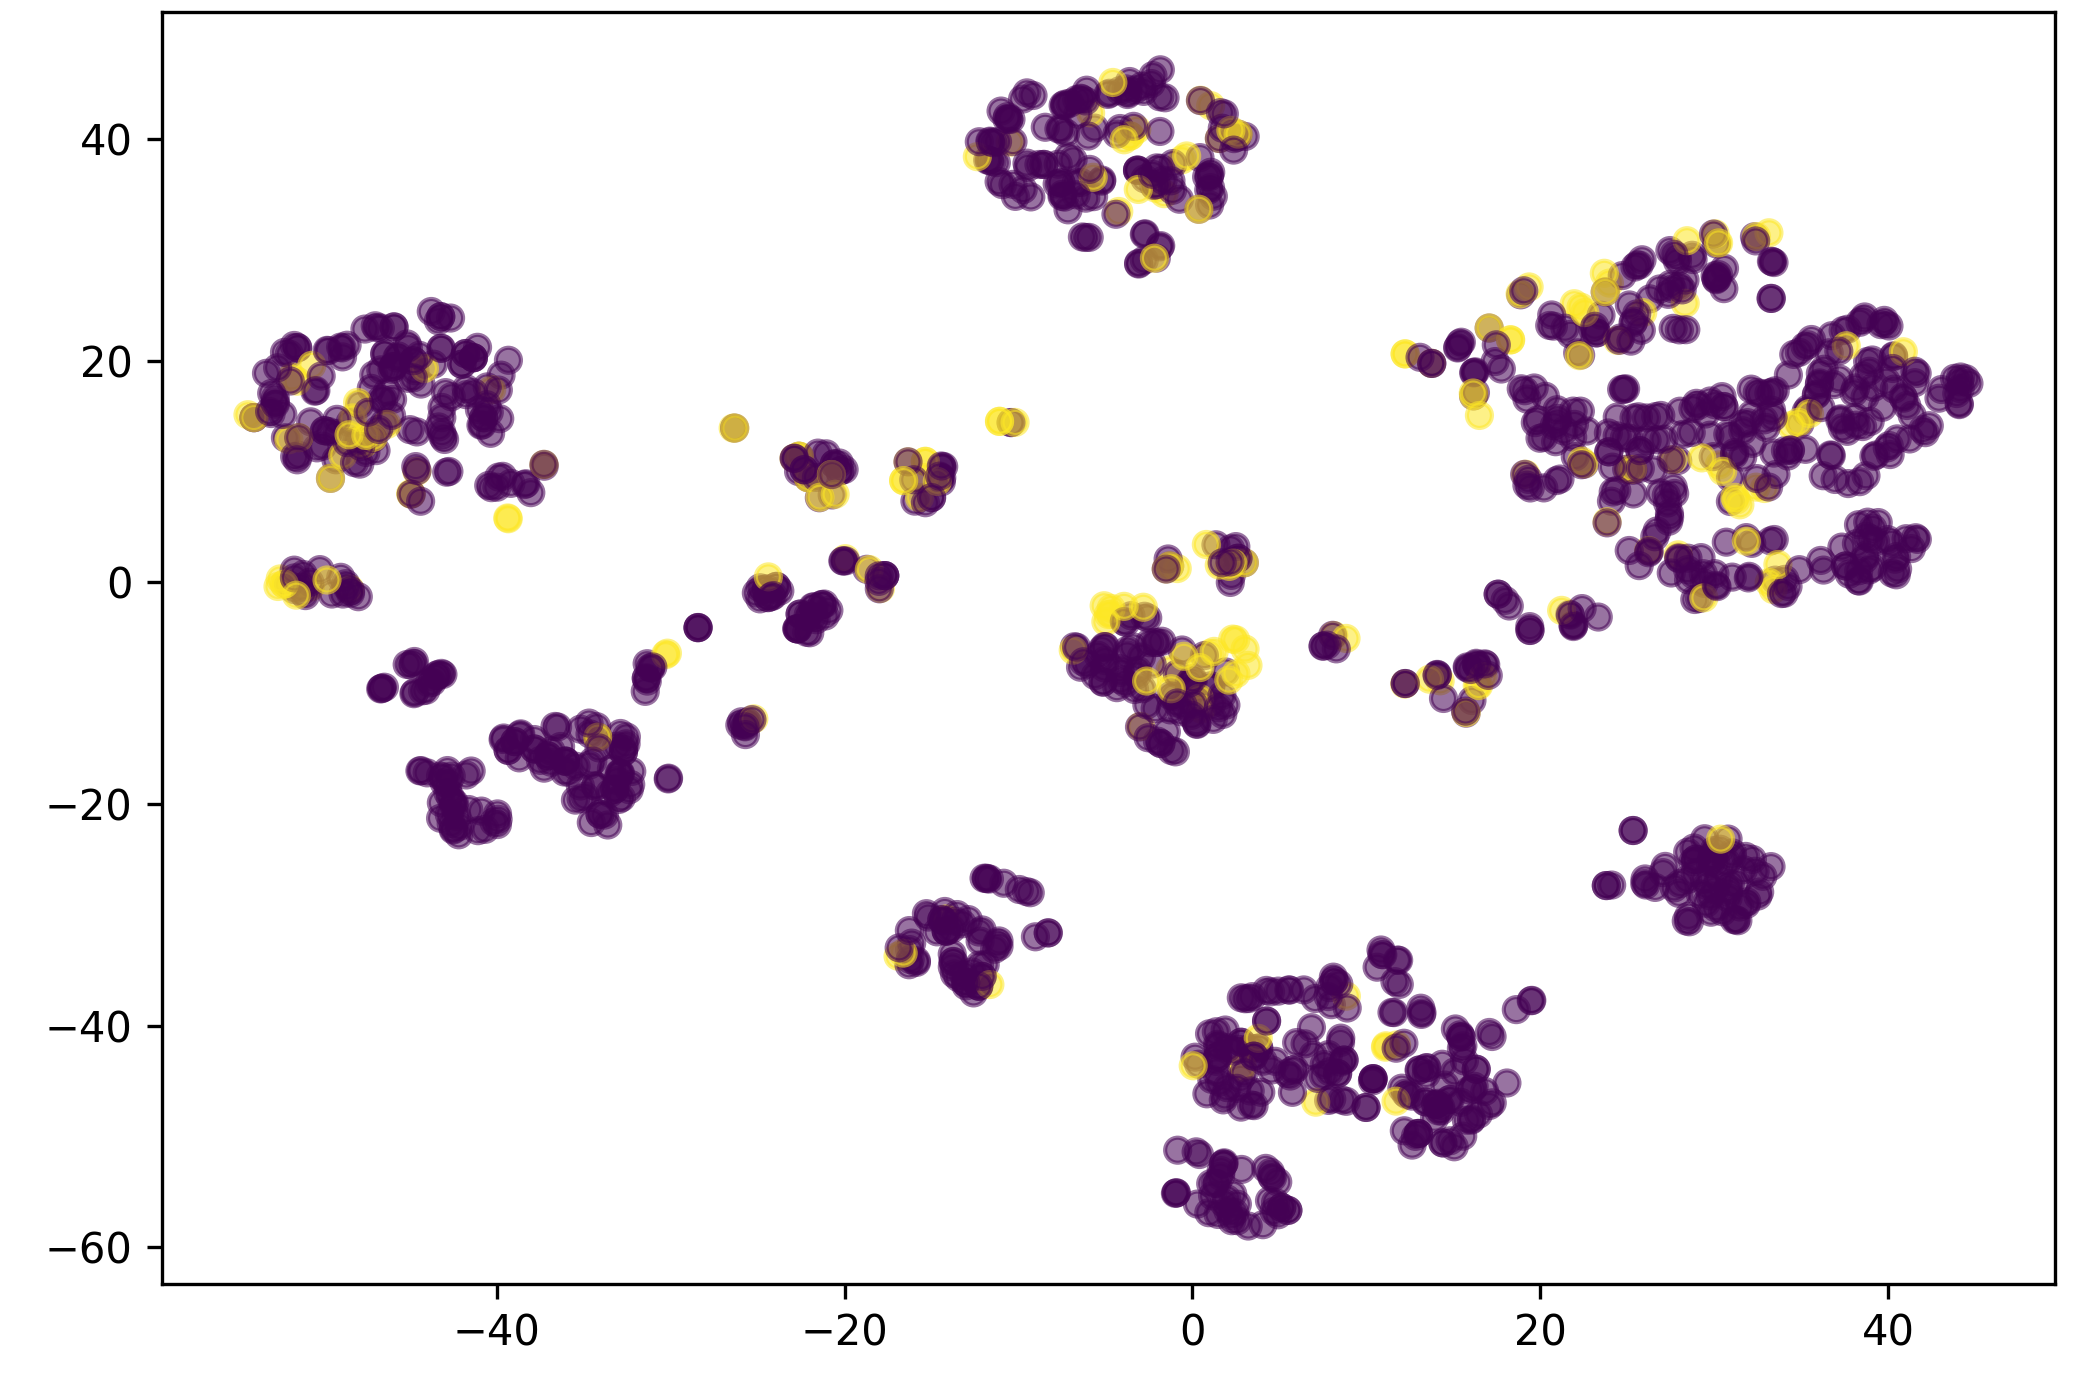
\includegraphics[keepaspectratio]{./media/image5.png}}

\textbf{Figure 5.} Two-dimensional t-SNE representation of the feature
space of the training set.

\pandocbounded{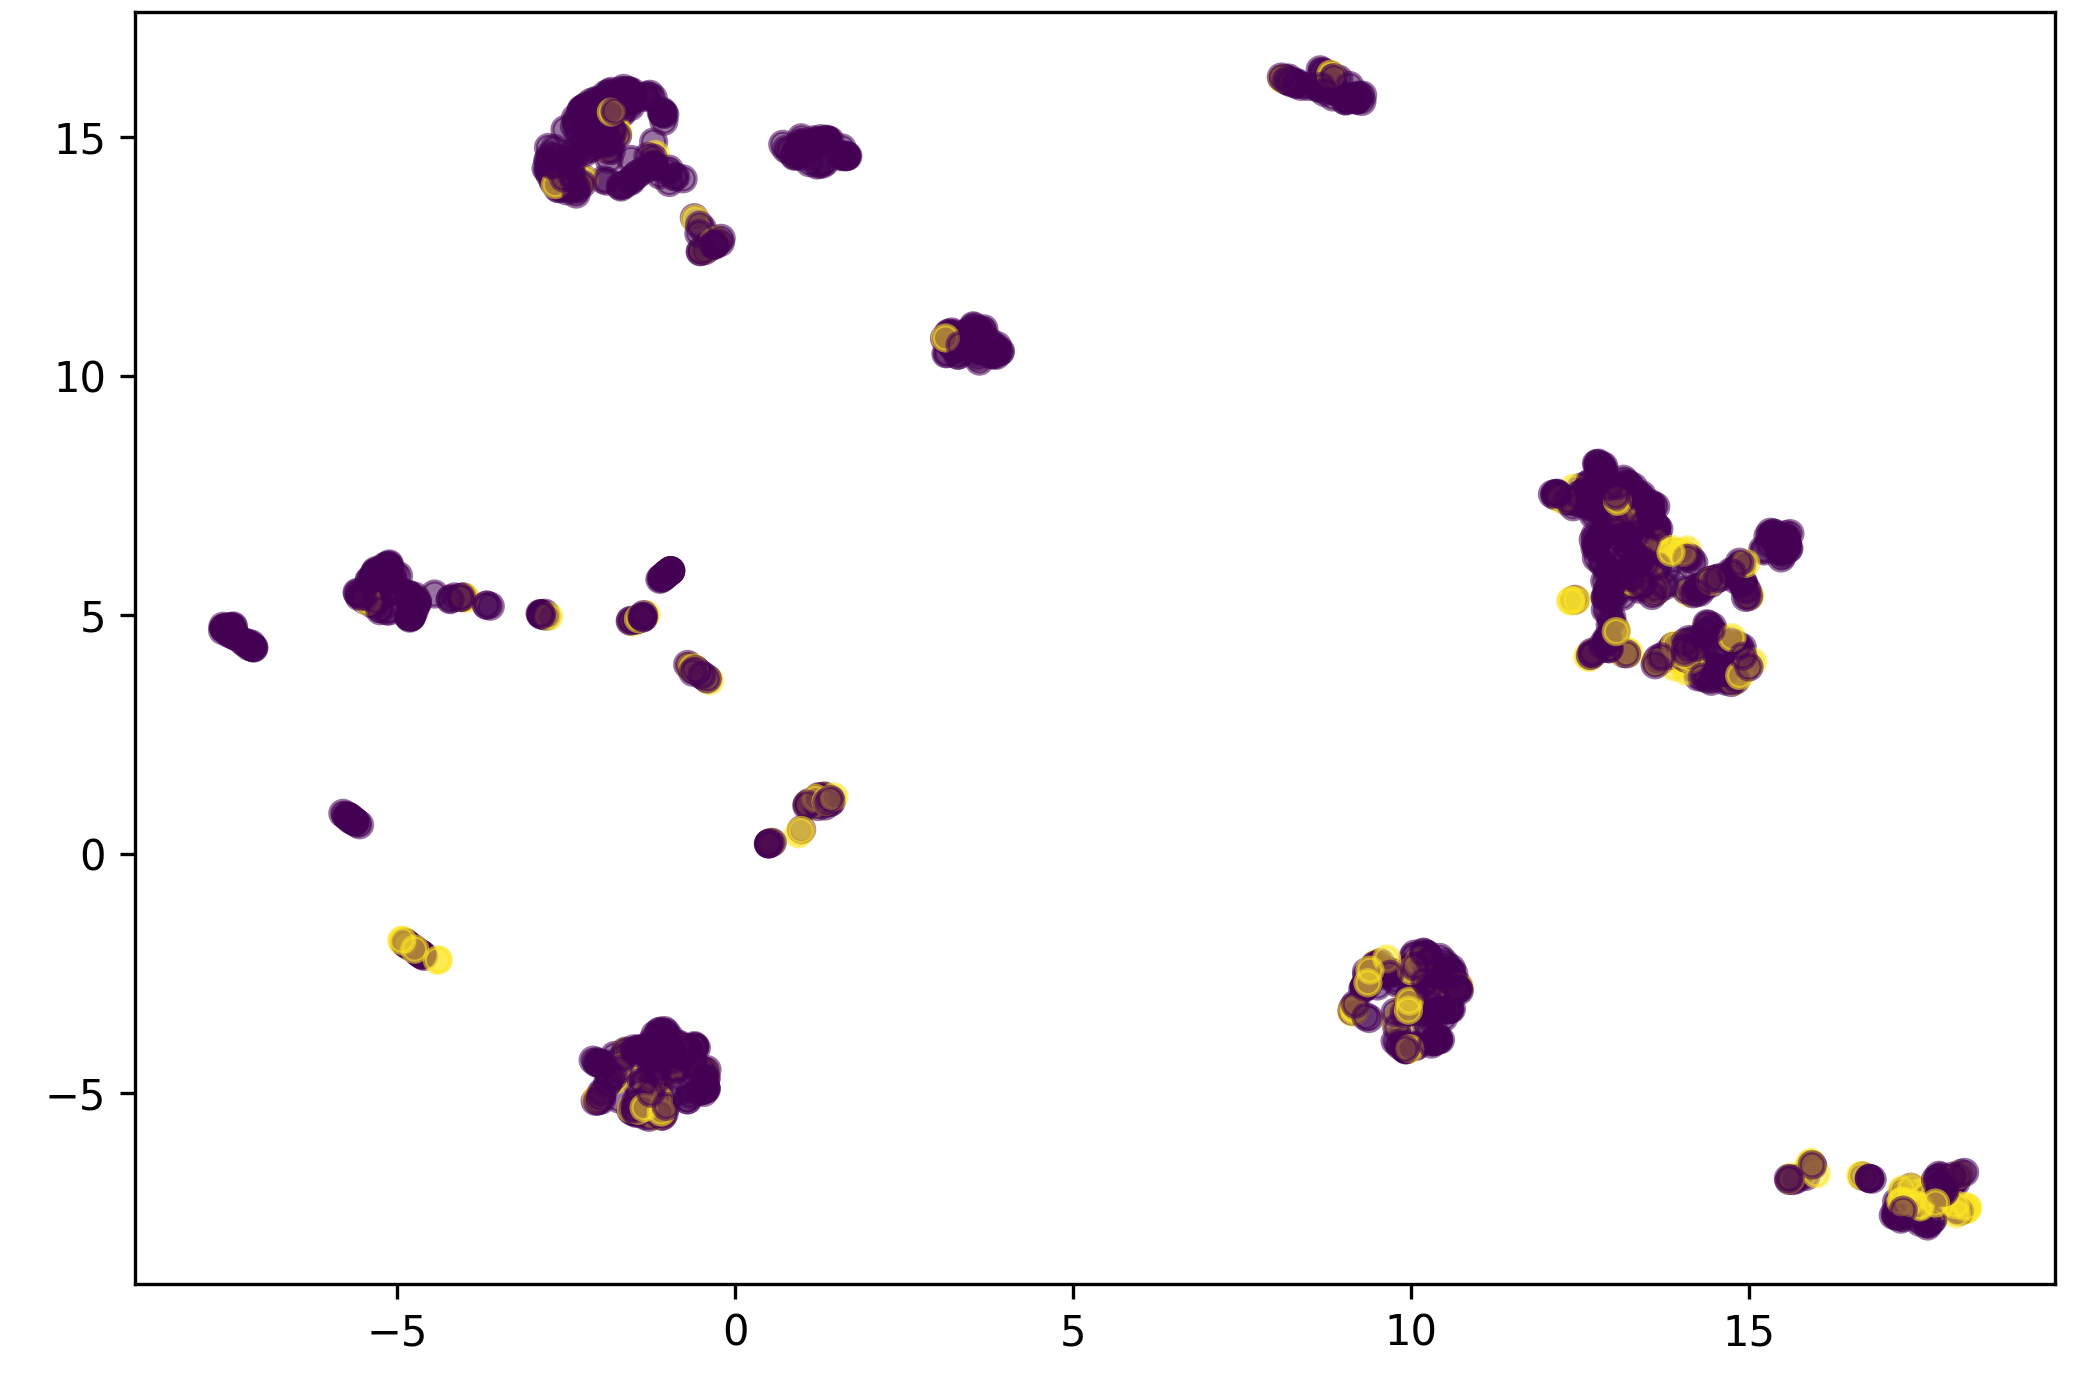
\includegraphics[keepaspectratio]{./media/image6.png}}

\textbf{Figure 6.} Two-dimensional UMAP representation of the feature
space of the training set.

The unsupervised validation (Table VII) corroborated this structure,
with K-Means (\emph{k} = 7) providing the partition with the highest
quality and stability compared with DBSCAN and Agglomerative clustering.

\textbf{TABLE VII.} SUMMARY OF THE UNSUPERVISED VALIDATION OF THE
FEATURE SPACE

{\def\LTcaptype{none} % do not increment counter
\begin{longtable}[]{@{}
  >{\raggedright\arraybackslash}p{(\linewidth - 4\tabcolsep) * \real{0.2055}}
  >{\raggedright\arraybackslash}p{(\linewidth - 4\tabcolsep) * \real{0.4041}}
  >{\raggedright\arraybackslash}p{(\linewidth - 4\tabcolsep) * \real{0.3767}}@{}}
\toprule\noalign{}
\begin{minipage}[b]{\linewidth}\raggedright
\textbf{Analysis}
\end{minipage} & \begin{minipage}[b]{\linewidth}\raggedright
\textbf{Evidence}
\end{minipage} & \begin{minipage}[b]{\linewidth}\raggedright
\textbf{Result + Interpretation}
\end{minipage} \\
\midrule\noalign{}
\endhead
\bottomrule\noalign{}
\endlastfoot
PCA (2 Components) & Fig. 4 & Global organization; partial nonlinear
separation \\
t-SNE & Fig. 5 & Compact local clusters; nonlinear relationships \\
UMAP & Fig. 6 & Stable structure; consistent multivariate patterns \\
K-Means & Silh = 0.262; DB = 1.507; CH = 1173.6; ARI = 0.77 ± 0.13 &
Optimal (K = 7); robustness confirmed by bootstrap \\
DBSCAN & 46 clusters; Silh = 0.161; DB = 1.310; CH = 245.9 &
Exploratory; fragmented partition with lower quality \\
Agglomerative Clustering & Silh = 0.250 ((k = 5)); DB = 1.573; CH =
1273.8 & Exploratory; lower quality than K-Means \\
Isolation Forest & 51/6076 (0.84\%) & Low proportion; no large-scale
anomalies \\
Local Outlier Factor & 54/6076 (0.89\%) & Consistent with the training
set \\
Robust Mahalanobis Distance & 152/6076 (2.50\%) & No extreme outliers \\
\end{longtable}
}

\subsection{D. Experimental Design}\label{d.-experimental-design}

The methodological workflow of the experimental design is illustrated in
Figure 7 and described throughout this section.

\pandocbounded{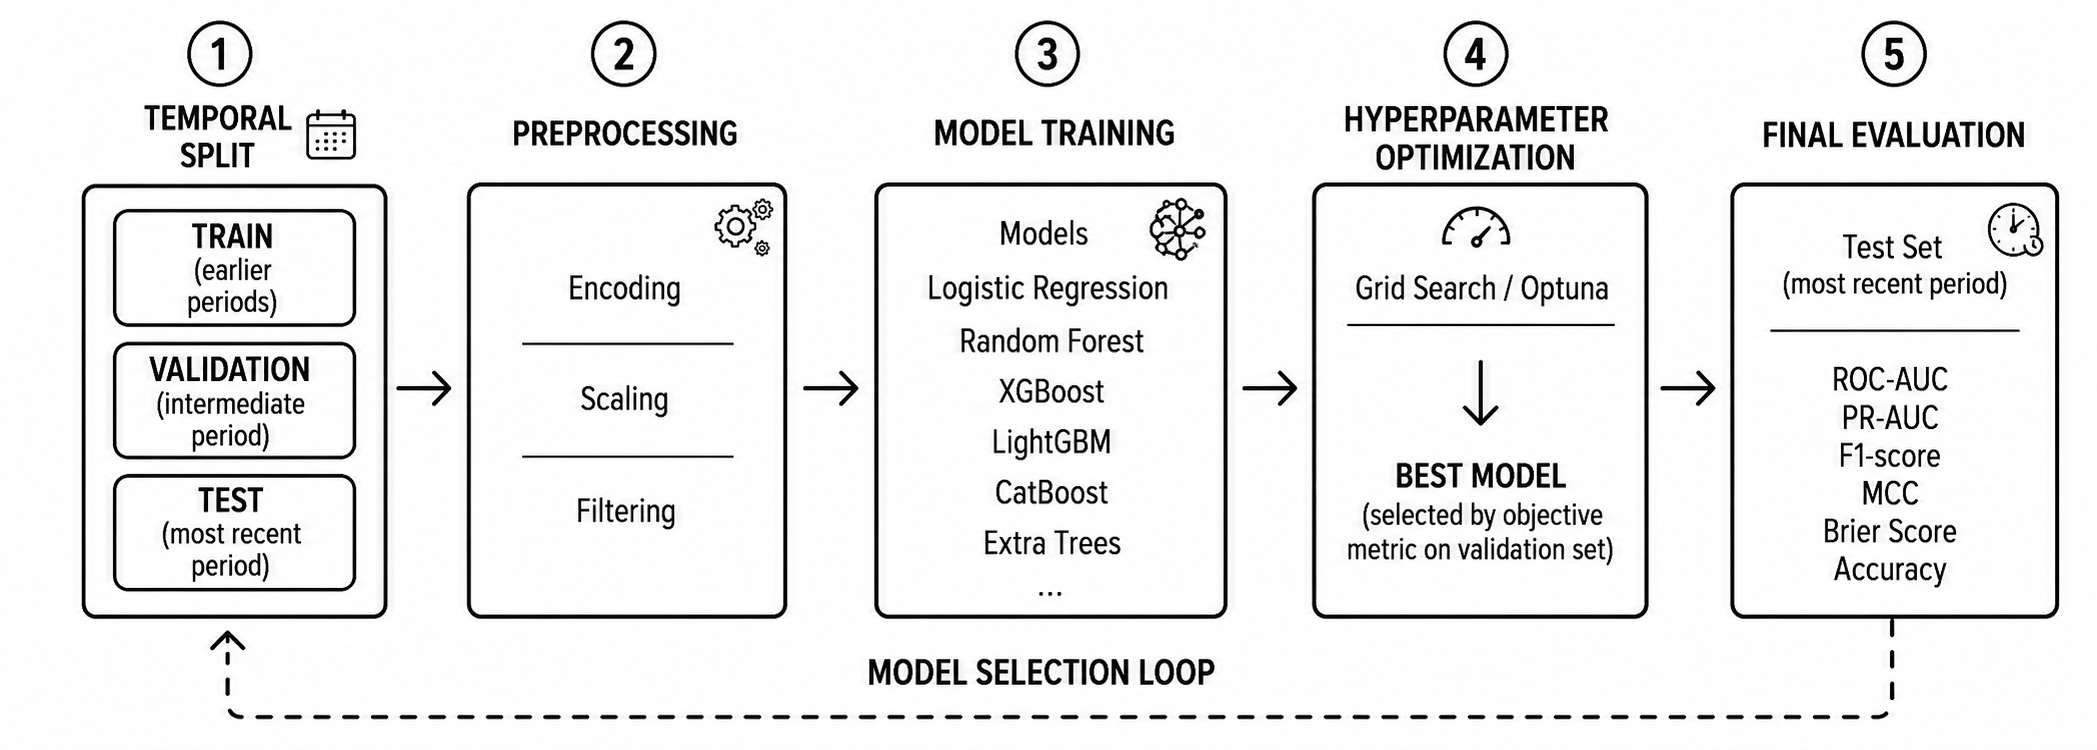
\includegraphics[keepaspectratio]{./media/image7.png}}

\textbf{Figure 7.} Experimental design for model training and temporal
validation.

\subsubsection{1) Temporal Data
Partitioning}\label{temporal-data-partitioning}

The experimental design replaces conventional random cross-validation
with a cumulative chronological strategy based on annual blocks
(year-block walk-forward validation).

Within the primary training block (2019--2023), sequential folds are
organized chronologically. At each iteration, the model is trained
exclusively using data from periods preceding the year under internal
evaluation.

Externally, the 2024 period was isolated as the validation and
calibration set (for classifier selection and optimal threshold
determination); the 2025 observations were reserved as the final
hold-out test set; and the partial 2026 segment was used as an
independent prospective evaluation set. None of these three temporal
horizons participated in the hyperparameter optimization process.

\subsubsection{2) Model Configurations}\label{model-configurations}

Nine algorithmic configurations were evaluated (Table VIII), including
one baseline classifier, two linear/margin-based models (SVM calibrated
using \emph{CalibratedClassifierCV}), three gradient boosting
architectures, one Bayesian-optimized LightGBM variant, and two ensemble
meta-models (Section III.D.2).

\textbf{TABLE VIII.} MODEL CONFIGURATIONS EVALUATED (HYPERPARAMETER
SEARCH)

{\def\LTcaptype{none} % do not increment counter
\begin{longtable}[]{@{}
  >{\raggedright\arraybackslash}p{(\linewidth - 6\tabcolsep) * \real{0.2476}}
  >{\raggedright\arraybackslash}p{(\linewidth - 6\tabcolsep) * \real{0.4190}}
  >{\raggedright\arraybackslash}p{(\linewidth - 6\tabcolsep) * \real{0.2286}}
  >{\raggedright\arraybackslash}p{(\linewidth - 6\tabcolsep) * \real{0.0857}}@{}}
\toprule\noalign{}
\begin{minipage}[b]{\linewidth}\raggedright
\textbf{Model}
\end{minipage} & \begin{minipage}[b]{\linewidth}\raggedright
\textbf{Optimizer}
\end{minipage} & \begin{minipage}[b]{\linewidth}\raggedright
\textbf{No.~of Iterations}
\end{minipage} & \begin{minipage}[b]{\linewidth}\raggedright
\textbf{F1}
\end{minipage} \\
\midrule\noalign{}
\endhead
\bottomrule\noalign{}
\endlastfoot
Dummy & --- & --- & --- \\
Logistic Regression & RandomizedSearchCV & 100 & 0.485 \\
SVM (LinearSVC + Platt) & RandomizedSearchCV & 100 & 0.268 \\
XGBoost & RandomizedSearchCV & 100 & 0.553 \\
LightGBM & RandomizedSearchCV & 100 & 0.563 \\
CatBoost & RandomizedSearchCV & 100 & 0.563 \\
LightGBM (Optuna) & TPE (Optuna) & 100 & 0.568 \\
VotingClassifier & --- (Ensemble, No Hyperparameter Tuning) & --- &
--- \\
Temporal Stacking & --- (Meta-Model Based on OOF Predictions) & --- &
--- \\
\end{longtable}
}

Note: The complete hyperparameter search spaces for all models are
provided in the associated code repository.

To mitigate the native class imbalance of the dataset (86\% versus
14\%), compatible models incorporated internal penalization techniques
through class weighting in their loss functions (\emph{class\_weight =
"balanced"} or \emph{scale\_pos\_weight}), while synthetic resampling
was omitted because the observed imbalance did not require an artificial
expansion of the sample space.

Based on this configuration, two meta-models were constructed by
combining the five base estimators with the highest internal
cross-validation F1 scores---Logistic Regression, LightGBM,
Optuna-optimized LightGBM, XGBoost, and CatBoost, excluding SVM because
of its lower performance (CV F1 = 0.268): a soft voting ensemble
(\emph{VotingClassifier}), which computes the unweighted average of the
predicted probabilities from the five models (Eq. (3)), and a temporal
stacking classifier (\emph{Stacking}), which trains a Logistic
Regression model using the five out-of-fold probabilities as
meta-features (Eq. (4), Section III.D.3).

\[\hat{p}(y=1 \mid x) = \frac{1}{5}\sum_{k=1}^{5}\hat{p}_k(y=1 \mid x) \tag{3}\]

\subsubsection{3) Optimization Strategy}\label{optimization-strategy}

The hyperparameters of the base estimators were tuned using
\emph{RandomizedSearchCV} (N = 100 iterations), maximizing the F1-score
metric over the temporal folds defined previously.

The LightGBM architecture was explored using Bayesian optimization (TPE
in \emph{Optuna}, 100 trials), maximizing the interannual F1-score as a
comparative configuration (Table VIII); however, the final selected
model was LightGBM optimized with \emph{RandomizedSearchCV}, as it
achieved a higher F1-score on the 2024 validation set (Table X).

The stacking meta-model (Logistic Regression) is trained on the
out-of-fold probabilities generated by the five base models as
meta-features (Eq. (4)).

\[\hat{p}_{\text{stack}}(y=1 \mid x_i) = \sigma\left(w^{\top} z_i + b\right), \quad z_i = \left[\hat{p}_1(x_i), \ldots, \hat{p}_5(x_i)\right] \tag{4}\]

where (\textbackslash sigma) denotes the logistic function, and (w) and
(b) are the parameters estimated by Logistic Regression.

This training was performed exclusively on the out-of-fold predictions
of the five base models across four temporal folds, thereby avoiding
overfitting bias. For inference, the base models were retrained using
the entire training set while keeping the meta-model fixed.

\subsubsection{4) Evaluation Protocol}\label{evaluation-protocol}

The proposed classifier was selected after comparing the F1-score and
ROC-AUC metrics on the 2024 validation block, with LightGBM identified
as the primary model.

The decision threshold was calibrated through a fine-grained grid search
(91 values within the range {[}0.05, 0.95{]}), maximizing the F1-score
on the validation set, which yielded an optimal cutoff of
(\textbackslash tau = 0.66). In parallel, alternative thresholds
(Youden\textquotesingle s J index, target precision, and target recall)
were estimated for operational sensitivity analysis.

The final predictive performance was formally reported on the 2025 test
set and the 2026 exploratory block using an extended set of evaluation
metrics: accuracy, precision, recall, F1-score, ROC-AUC, PR-AUC,
balanced accuracy, specificity, Matthews correlation coefficient (MCC),
Cohen\textquotesingle s kappa, negative predictive value (NPV), false
positive rate (FPR), false negative rate (FNR), and likelihood ratios
(LR+ and LR−).

All estimators were complemented with 95\% confidence intervals obtained
through bootstrap resampling, probabilistic calibration curves, and
temporal feature drift analysis using the Population Stability Index
(PSI) with respect to the baseline training block.

\textbf{TABLE IX.} PERFORMANCE OF THE FINAL MODEL (LIGHTGBM, THRESHOLD =
0.66) ACROSS TEMPORAL PARTITIONS

{\def\LTcaptype{none} % do not increment counter
\begin{longtable}[]{@{}
  >{\raggedright\arraybackslash}p{(\linewidth - 6\tabcolsep) * \real{0.4059}}
  >{\raggedright\arraybackslash}p{(\linewidth - 6\tabcolsep) * \real{0.2178}}
  >{\raggedright\arraybackslash}p{(\linewidth - 6\tabcolsep) * \real{0.1584}}
  >{\raggedright\arraybackslash}p{(\linewidth - 6\tabcolsep) * \real{0.1980}}@{}}
\toprule\noalign{}
\endhead
\bottomrule\noalign{}
\endlastfoot
\textbf{Metric} & \textbf{Validation 2024} & \textbf{Test 2025} &
\textbf{External 2026} \\
Accuracy & 0.890 & 0.862 & 0.842 \\
Precision & 0.576 & 0.525 & 0.644 \\
Recall & 0.667 & 0.424 & 0.493 \\
F1-score & 0.618 & 0.469 & 0.559 \\
ROC-AUC & 0.897 & 0.798 & 0.866 \\
PR-AUC & 0.625 & 0.499 & 0.652 \\
Matthews Correlation Coefficient (MCC) & 0.556 & 0.394 & 0.471 \\
Specificity & 0.925 & 0.936 & 0.931 \\
\end{longtable}
}

\section{IV. Results}\label{iv.-results}

\subsection{A. Comparison of Base Models and
Ensembles}\label{a.-comparison-of-base-models-and-ensembles}

Table X summarizes the performance of the six base models and the two
ensemble methods (\emph{VotingClassifier} and temporal \emph{Stacking})
on the 2024 validation set and the 2025 test set, using a fixed decision
threshold of 0.5.

\textbf{TABLE X.} MODEL COMPARISON (THRESHOLD = 0.5)

{\def\LTcaptype{none} % do not increment counter
\begin{longtable}[]{@{}
  >{\raggedright\arraybackslash}p{(\linewidth - 6\tabcolsep) * \real{0.3750}}
  >{\raggedright\arraybackslash}p{(\linewidth - 6\tabcolsep) * \real{0.2273}}
  >{\raggedright\arraybackslash}p{(\linewidth - 6\tabcolsep) * \real{0.1591}}
  >{\raggedright\arraybackslash}p{(\linewidth - 6\tabcolsep) * \real{0.2159}}@{}}
\toprule\noalign{}
\begin{minipage}[b]{\linewidth}\raggedright
\textbf{Model}
\end{minipage} & \begin{minipage}[b]{\linewidth}\raggedright
\textbf{Validation F1}
\end{minipage} & \begin{minipage}[b]{\linewidth}\raggedright
\textbf{Test F1}
\end{minipage} & \begin{minipage}[b]{\linewidth}\raggedright
\textbf{Test ROC-AUC}
\end{minipage} \\
\midrule\noalign{}
\endhead
\bottomrule\noalign{}
\endlastfoot
LightGBM (Randomized SearchCV) & 0.605 & 0.475 & 0.798 \\
CatBoost & 0.591 & 0.485 & 0.817 \\
XGBoost & 0.598 & 0.465 & 0.772 \\
Logistic Regression & 0.437 & 0.444 & 0.799 \\
SVM (LinearSVC + Platt) & 0.263 & 0.247 & 0.803 \\
VotingClassifier & 0.584 & 0.476 & 0.819 \\
Temporal Stacking & 0.518 & 0.445 & 0.822 \\
Dummy (Baseline) & 0.000 & 0.000 & 0.500 \\
\end{longtable}
}

The gradient boosting models consistently outperformed both the linear
models and the baseline classifier (F1 = 0 across all partitions),
confirming the presence of a nonlinear predictive signal. LightGBM
achieved the highest F1-score on the validation set---the criterion used
to select the primary model---whereas CatBoost outperformed LightGBM on
the 2025 test set in terms of both F1-score and ROC-AUC. This difference
was confirmed to be statistically significant by
DeLong\textquotesingle s test ((z = 2.70), (p = 0.007)). The Friedman
test across the temporal folds also confirmed significant overall
differences among the evaluated models ((\textbackslash chi\^{}2 =
12.6), (p = 0.013)).

Although CatBoost achieved a significantly higher F1-score on the test
set (DeLong\textquotesingle s test, *z* = 2.70, *p* = 0.007), selecting
the final model based on this result would have compromised the temporal
isolation established in Section III.D.1 by turning the 2025 hold-out
set into a model selection criterion rather than an independent
evaluation. Therefore, LightGBM was retained as the primary model
because it achieved the best performance under the pre-specified 2024
validation criterion (Section III.D.4). This decision is further
supported by its greater relative stability across the evaluated
temporal partitions (mean F1 = 0.541 ± 0.045 versus 0.528 ± 0.040 for
CatBoost; Section IV.B).

\subsection{B. Decision Threshold Optimization and Final Model
Performance}\label{b.-decision-threshold-optimization-and-final-model-performance}

After selecting LightGBM as the primary model and optimizing the
decision threshold on the validation set (F1-optimal = 0.66; Section
III.D.4), the final performance is presented in Table IX (Section
III.D): F1 = 0.618 on the validation set, 0.469 on the test set, and
0.559 on the 2026 external dataset, with 95\% confidence intervals
obtained through bootstrap resampling (300 resamples) of F1 ∈ {[}0.390,
0.546{]} on the test set.

External walk-forward cross-validation (incrementally retraining the
model year by year) confirmed the relative stability of LightGBM (mean
F1 = 0.541 ± 0.045) compared with CatBoost (0.528 ± 0.040) and Logistic
Regression (0.461 ± 0.025) across the seven temporal evaluation points
(2020--2026).

\subsection{C. Ablation Study of Feature
Groups}\label{c.-ablation-study-of-feature-groups}

Table XI summarizes the ablation study conducted on the LightGBM model,
evaluating the impact of removing entire feature families on predictive
performance.

\textbf{TABLE XI.} ABLATION STUDY (LIGHTGBM, 2025 TEST SET)

{\def\LTcaptype{none} % do not increment counter
\begin{longtable}[]{@{}
  >{\raggedright\arraybackslash}p{(\linewidth - 12\tabcolsep) * \real{0.3083}}
  >{\raggedright\arraybackslash}p{(\linewidth - 12\tabcolsep) * \real{0.1250}}
  >{\raggedright\arraybackslash}p{(\linewidth - 12\tabcolsep) * \real{0.0750}}
  >{\raggedright\arraybackslash}p{(\linewidth - 12\tabcolsep) * \real{0.1083}}
  >{\raggedright\arraybackslash}p{(\linewidth - 12\tabcolsep) * \real{0.1333}}
  >{\raggedright\arraybackslash}p{(\linewidth - 12\tabcolsep) * \real{0.1167}}
  >{\raggedright\arraybackslash}p{(\linewidth - 12\tabcolsep) * \real{0.1167}}@{}}
\toprule\noalign{}
\begin{minipage}[b]{\linewidth}\raggedright
\textbf{Variant}
\end{minipage} & \begin{minipage}[b]{\linewidth}\raggedright
\textbf{No.~vars}
\end{minipage} & \begin{minipage}[b]{\linewidth}\raggedright
\textbf{F1}
\end{minipage} & \begin{minipage}[b]{\linewidth}\raggedright
\textbf{Recall}
\end{minipage} & \begin{minipage}[b]{\linewidth}\raggedright
\textbf{Precision}
\end{minipage} & \begin{minipage}[b]{\linewidth}\raggedright
\textbf{ROC-AUC}
\end{minipage} & \begin{minipage}[b]{\linewidth}\raggedright
\textbf{PR-AUC}
\end{minipage} \\
\midrule\noalign{}
\endhead
\bottomrule\noalign{}
\endlastfoot
Full Model (69 Features) & 69 & 0.466 & 0.541 & 0.410 & 0.788 & 0.507 \\
Without Historical Growth Features & 66 & 0.471 & 0.552 & 0.411 & 0.810
& 0.521 \\
Without Frequency Encoding & 64 & 0.458 & 0.622 & 0.363 & 0.818 &
0.522 \\
Without Interaction Features & 26 & 0.415 & 0.634 & 0.309 & 0.778 &
0.348 \\
Without Territorial Features & 23 & 0.415 & 0.721 & 0.292 & 0.792 &
0.367 \\
\end{longtable}
}

The removal of categorical interaction features and territorial
attributes produced the largest decreases in F1-score observed in the
study (0.415 in both cases, compared with 0.466 for the full model).

Removing the territorial features shifted the model toward a less
selective behavior---increasing recall (0.541 → 0.721) at the expense of
a substantial reduction in precision (0.410 → 0.292)---whereas excluding
the categorical interaction features produced the largest decrease in
PR-AUC observed in the study (0.507 → 0.348). Overall, these results
indicate that the predictive signal depends primarily on the territorial
and institutional structure of the system rather than on the historical
variables considered in isolation.

In contrast, ROC-AUC remained stable or even improved slightly in both
variants (0.792 and 0.778 versus 0.788 for the full model), indicating
that the model\textquotesingle s probabilistic ranking capability is
resilient to the removal of these feature groups and that the observed
impact on F1-score is mainly attributable to the fixed decision
threshold (0.5) used in this experiment, which differs from the
calibrated threshold ((\textbackslash tau = 0.66)) adopted for the final
model.

By comparison, removing the historical growth features did not degrade
performance (F1 = 0.471), while removing frequency encoding produced
only a marginal variation in F1-score (0.458) together with an
improvement in ROC-AUC (0.818). These findings indicate informational
redundancy with the remaining territorial interaction blocks and
empirically validate the previous multicollinearity audit.

\subsection{D. Explainability: Global Feature
Importance}\label{d.-explainability-global-feature-importance}

Both permutation importance and the mean absolute SHAP values (Section
V) consistently identify the territorial-institutional frequency
variables and the \emph{tipo\_caso\_DENUNCIA} feature as the most
influential predictors, consistent with the findings of the ablation
study regarding the relevance of territorial features.

The SHAP interaction analysis identified the combination
\emph{freq\_inter\_distrito\_tipo\_caso} × \emph{ubigeo\_pjfs} as the
feature pair with the highest mean interaction value (0.108).
Furthermore, the controlled counterfactual analysis showed that, in
several individual cases, a single feature was sufficient to cross the
decision threshold, highlighting that the model is more sensitive to the
institutional typology of the case than to the accumulated historical
workload.

\subsection{E. Temporal Robustness and Uncertainty
Quantification}\label{e.-temporal-robustness-and-uncertainty-quantification}

Figure 8 shows that the model maintains adequate calibration for low
predicted probabilities, although it exhibits overconfidence in the
medium-to-high probability range (ECE = 0.091; MCE = 0.464).

Since the operational decision threshold ((\textbackslash tau = 0.66))
is located near this region, the predicted score should be interpreted
as a relative prioritization criterion rather than as an exactly
calibrated probability.

\pandocbounded{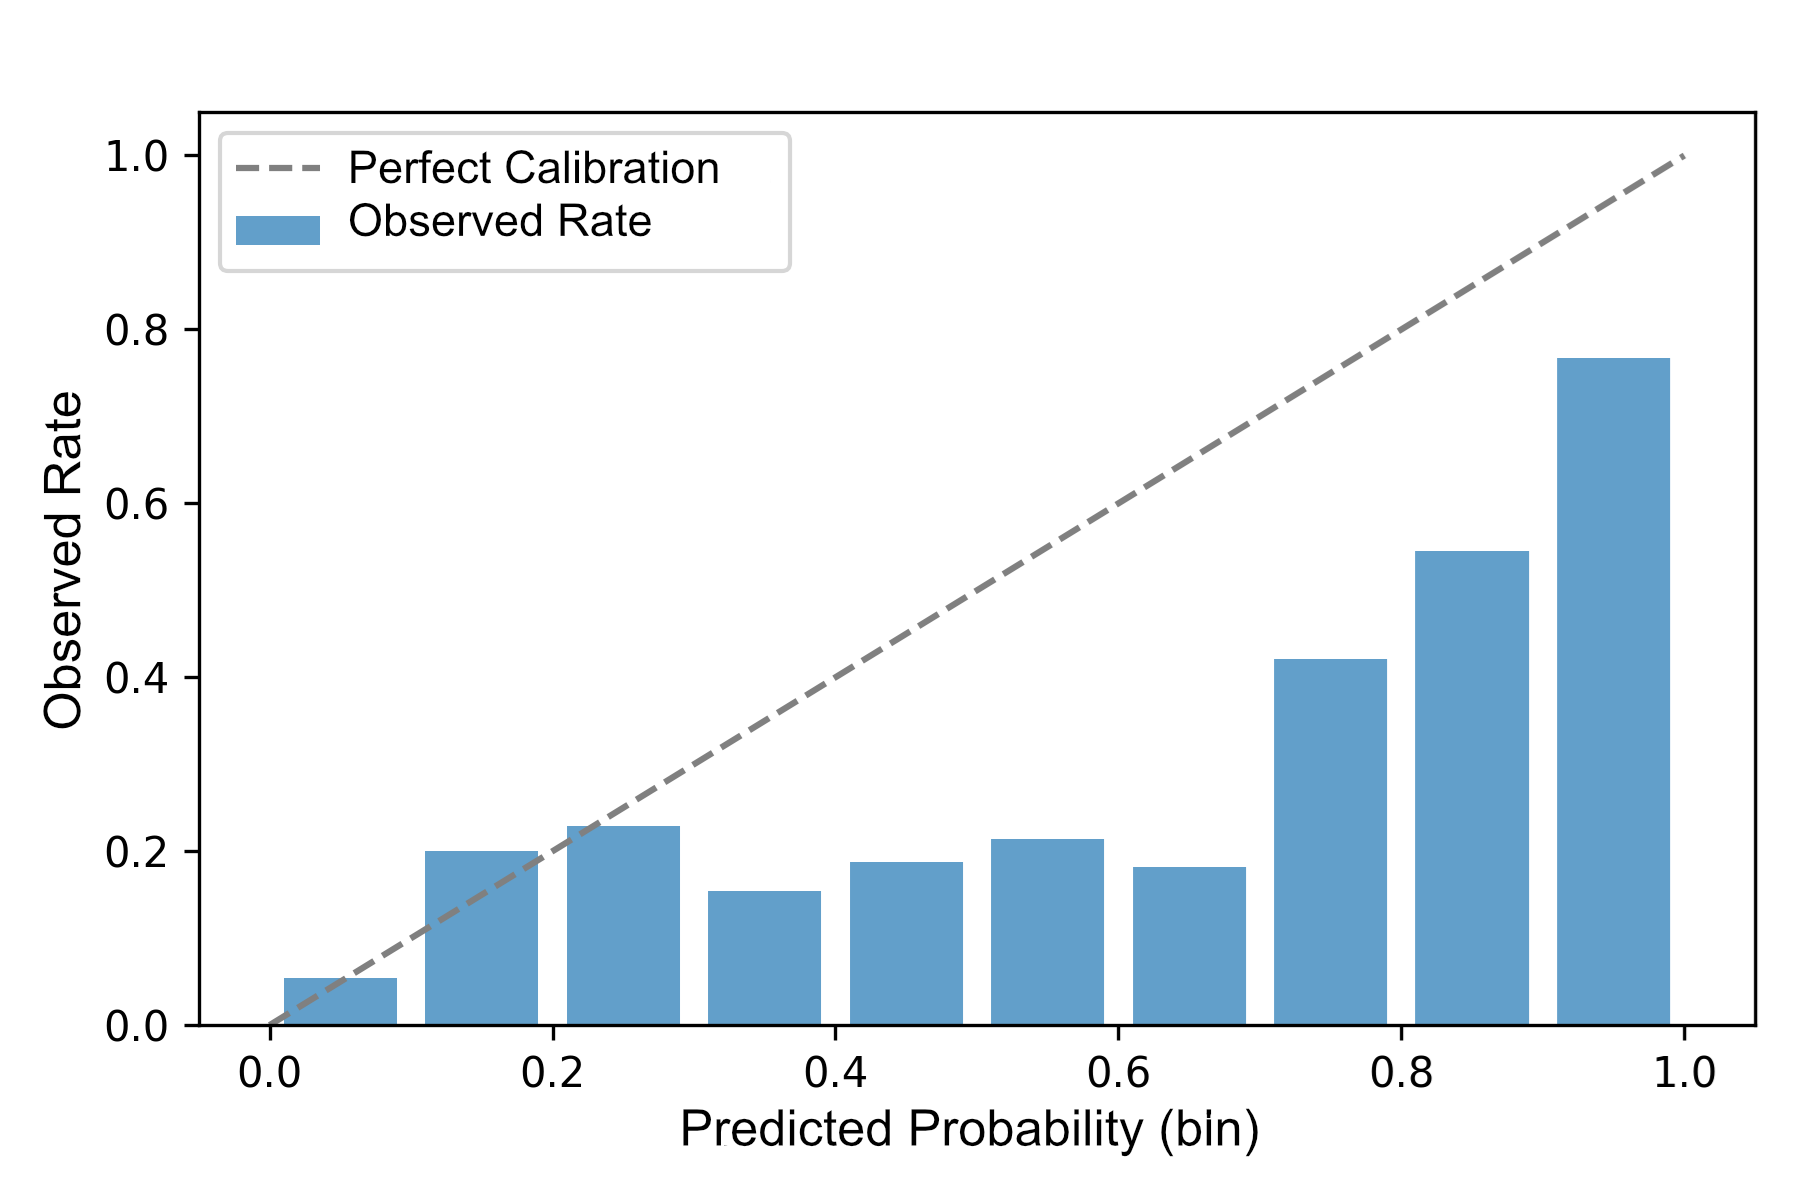
\includegraphics[keepaspectratio]{./media/image8.png}}

\textbf{Figure 8.} Reliability diagram of the final model (LightGBM, (τ=
0.66)) on the 2025 test set.

\subsection{F. Unsupervised Validation and Territorial
Fairness}\label{f.-unsupervised-validation-and-territorial-fairness}

The unsupervised validation confirmed that the clusters with the highest
average case backlog concentrated the highest proxy risk rates,
supporting the consistency between the identified operational structure
and the model predictions (Table VII).

The preliminary fairness audit identified performance differences across
prosecution office types and specialties. These differences should be
interpreted as indicators for institutional monitoring rather than as
evidence of causal discrimination, in accordance with the literature on
the limitations of risk assessment tools in the justice system
\citep{dressel_accuracy_2018}.

Overall, the calibration assessment, unsupervised structure analysis,
and fairness audit indicate that the model maintains stable behavior
under different validation criteria, reinforcing its reliability as a
decision-support tool for operational management.

\section{V. Interpretability And
Impact}\label{v.-interpretability-and-impact}

\subsection{A. Interpretability}\label{a.-interpretability}

The interpretability analysis is based exclusively on SHAP
\citep{lundberg_unified_2017}, applied to the final model on the 2025
test set. Figure 9 presents the global summary of the mean absolute SHAP
values for the most influential features.

Figure 9 shows that the model primarily bases its predictions on
territorial and institutional patterns rather than on isolated
historical variables.

In particular, the features associated with territorial organization,
institutional specialization, and operational frequency patterns account
for the greatest predictive contribution, suggesting that the proxy risk
reflects specific operational configurations of the Public
Prosecutor\textquotesingle s Office -- Office of the Attorney General of
Peru (MPFN) rather than the individual volume of operational
combinations.

Five features account for 53\% of the total SHAP signal, whereas the
remaining 50 features contribute only 6\%, indicating that the model
prioritizes operational patterns associated with case processing
frequency, territorial organization, and prosecutorial specialization.

By contrast, the historical features provide complementary information,
consistent with the ablation study (Table XI), which showed that
interaction features contributed more to predictive performance than
individual historical indicators.

\pandocbounded{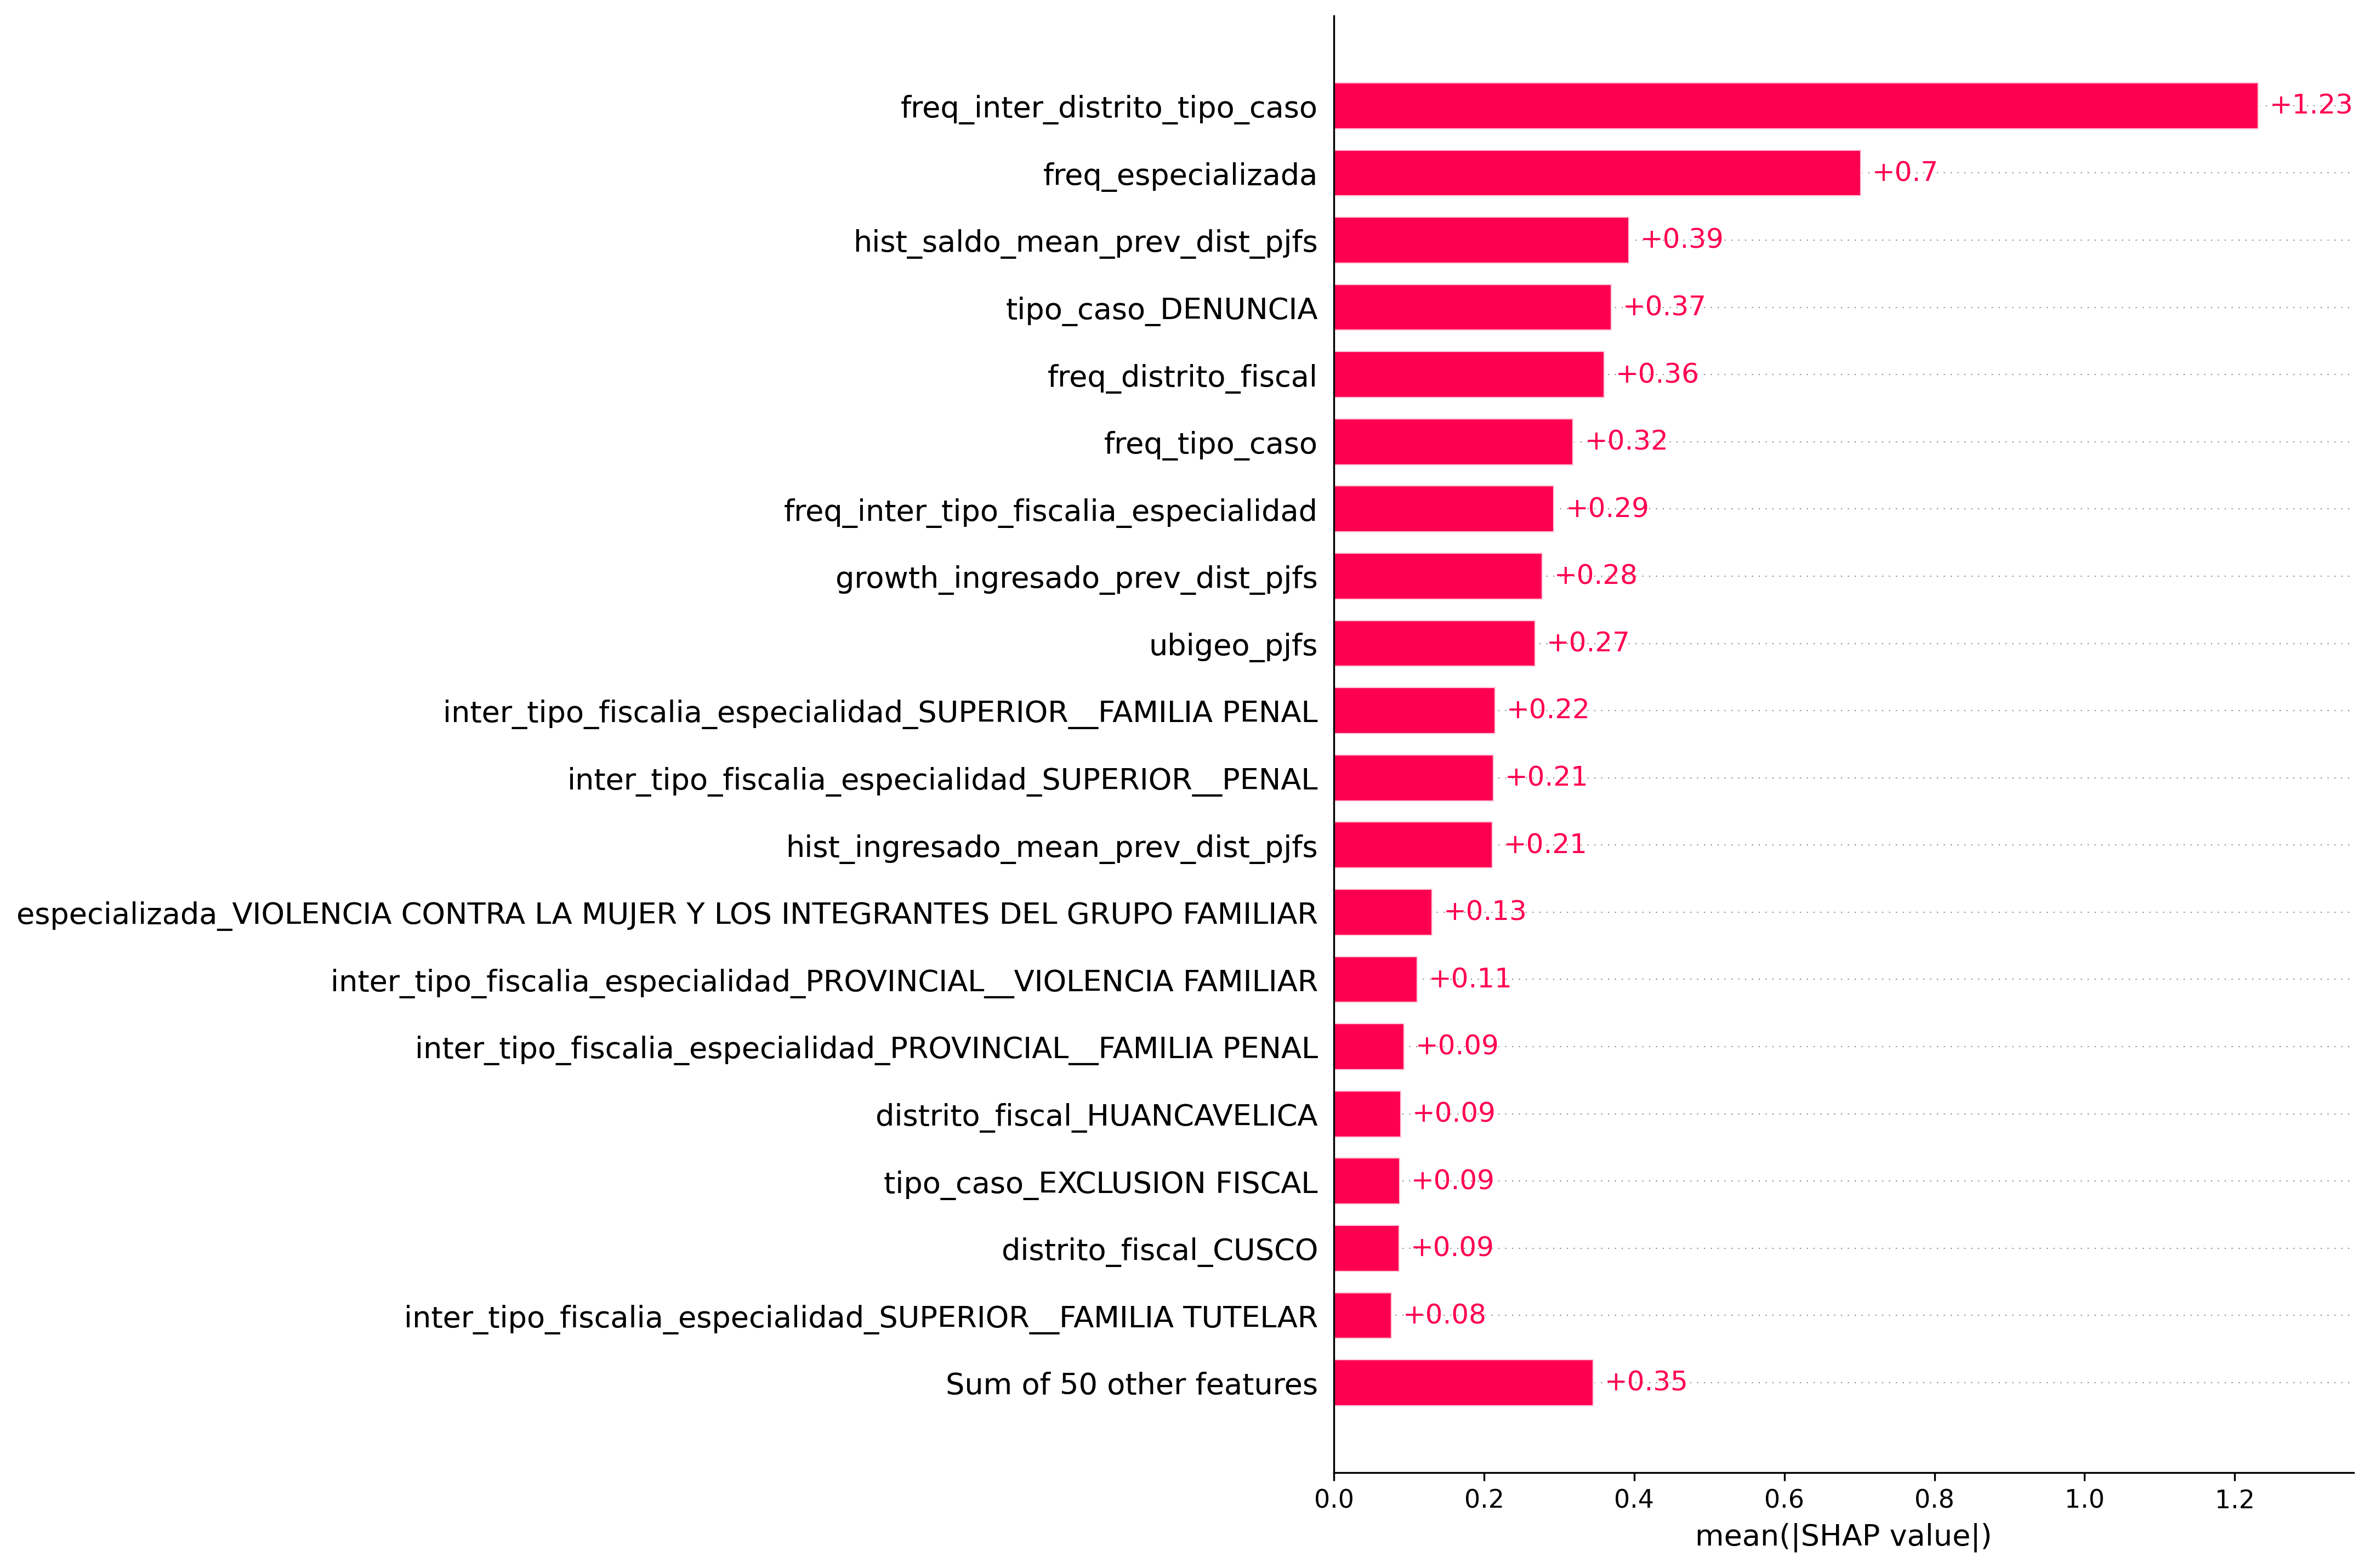
\includegraphics[keepaspectratio]{./media/image9.png}}

\textbf{Figure 9.} Global feature importance according to mean SHAP
values.

While Figure 9 summarizes the global importance of the features at the
model level, Figure 10 illustrates how these features contribute
positively or negatively to individual predictions, making it possible
to analyze the variability of their effects across different operational
combinations.

Whereas some features exhibit relatively stable contributions, others
show greater dispersion in their SHAP values, indicating that their
effect depends on the operational context and on their interaction with
other features within the operational combination. This behavior
reflects the nonlinear nature of the model and justifies the use of
interpretability tools to understand how different feature
configurations modify the predictions \citep{lundberg_unified_2017}.

\pandocbounded{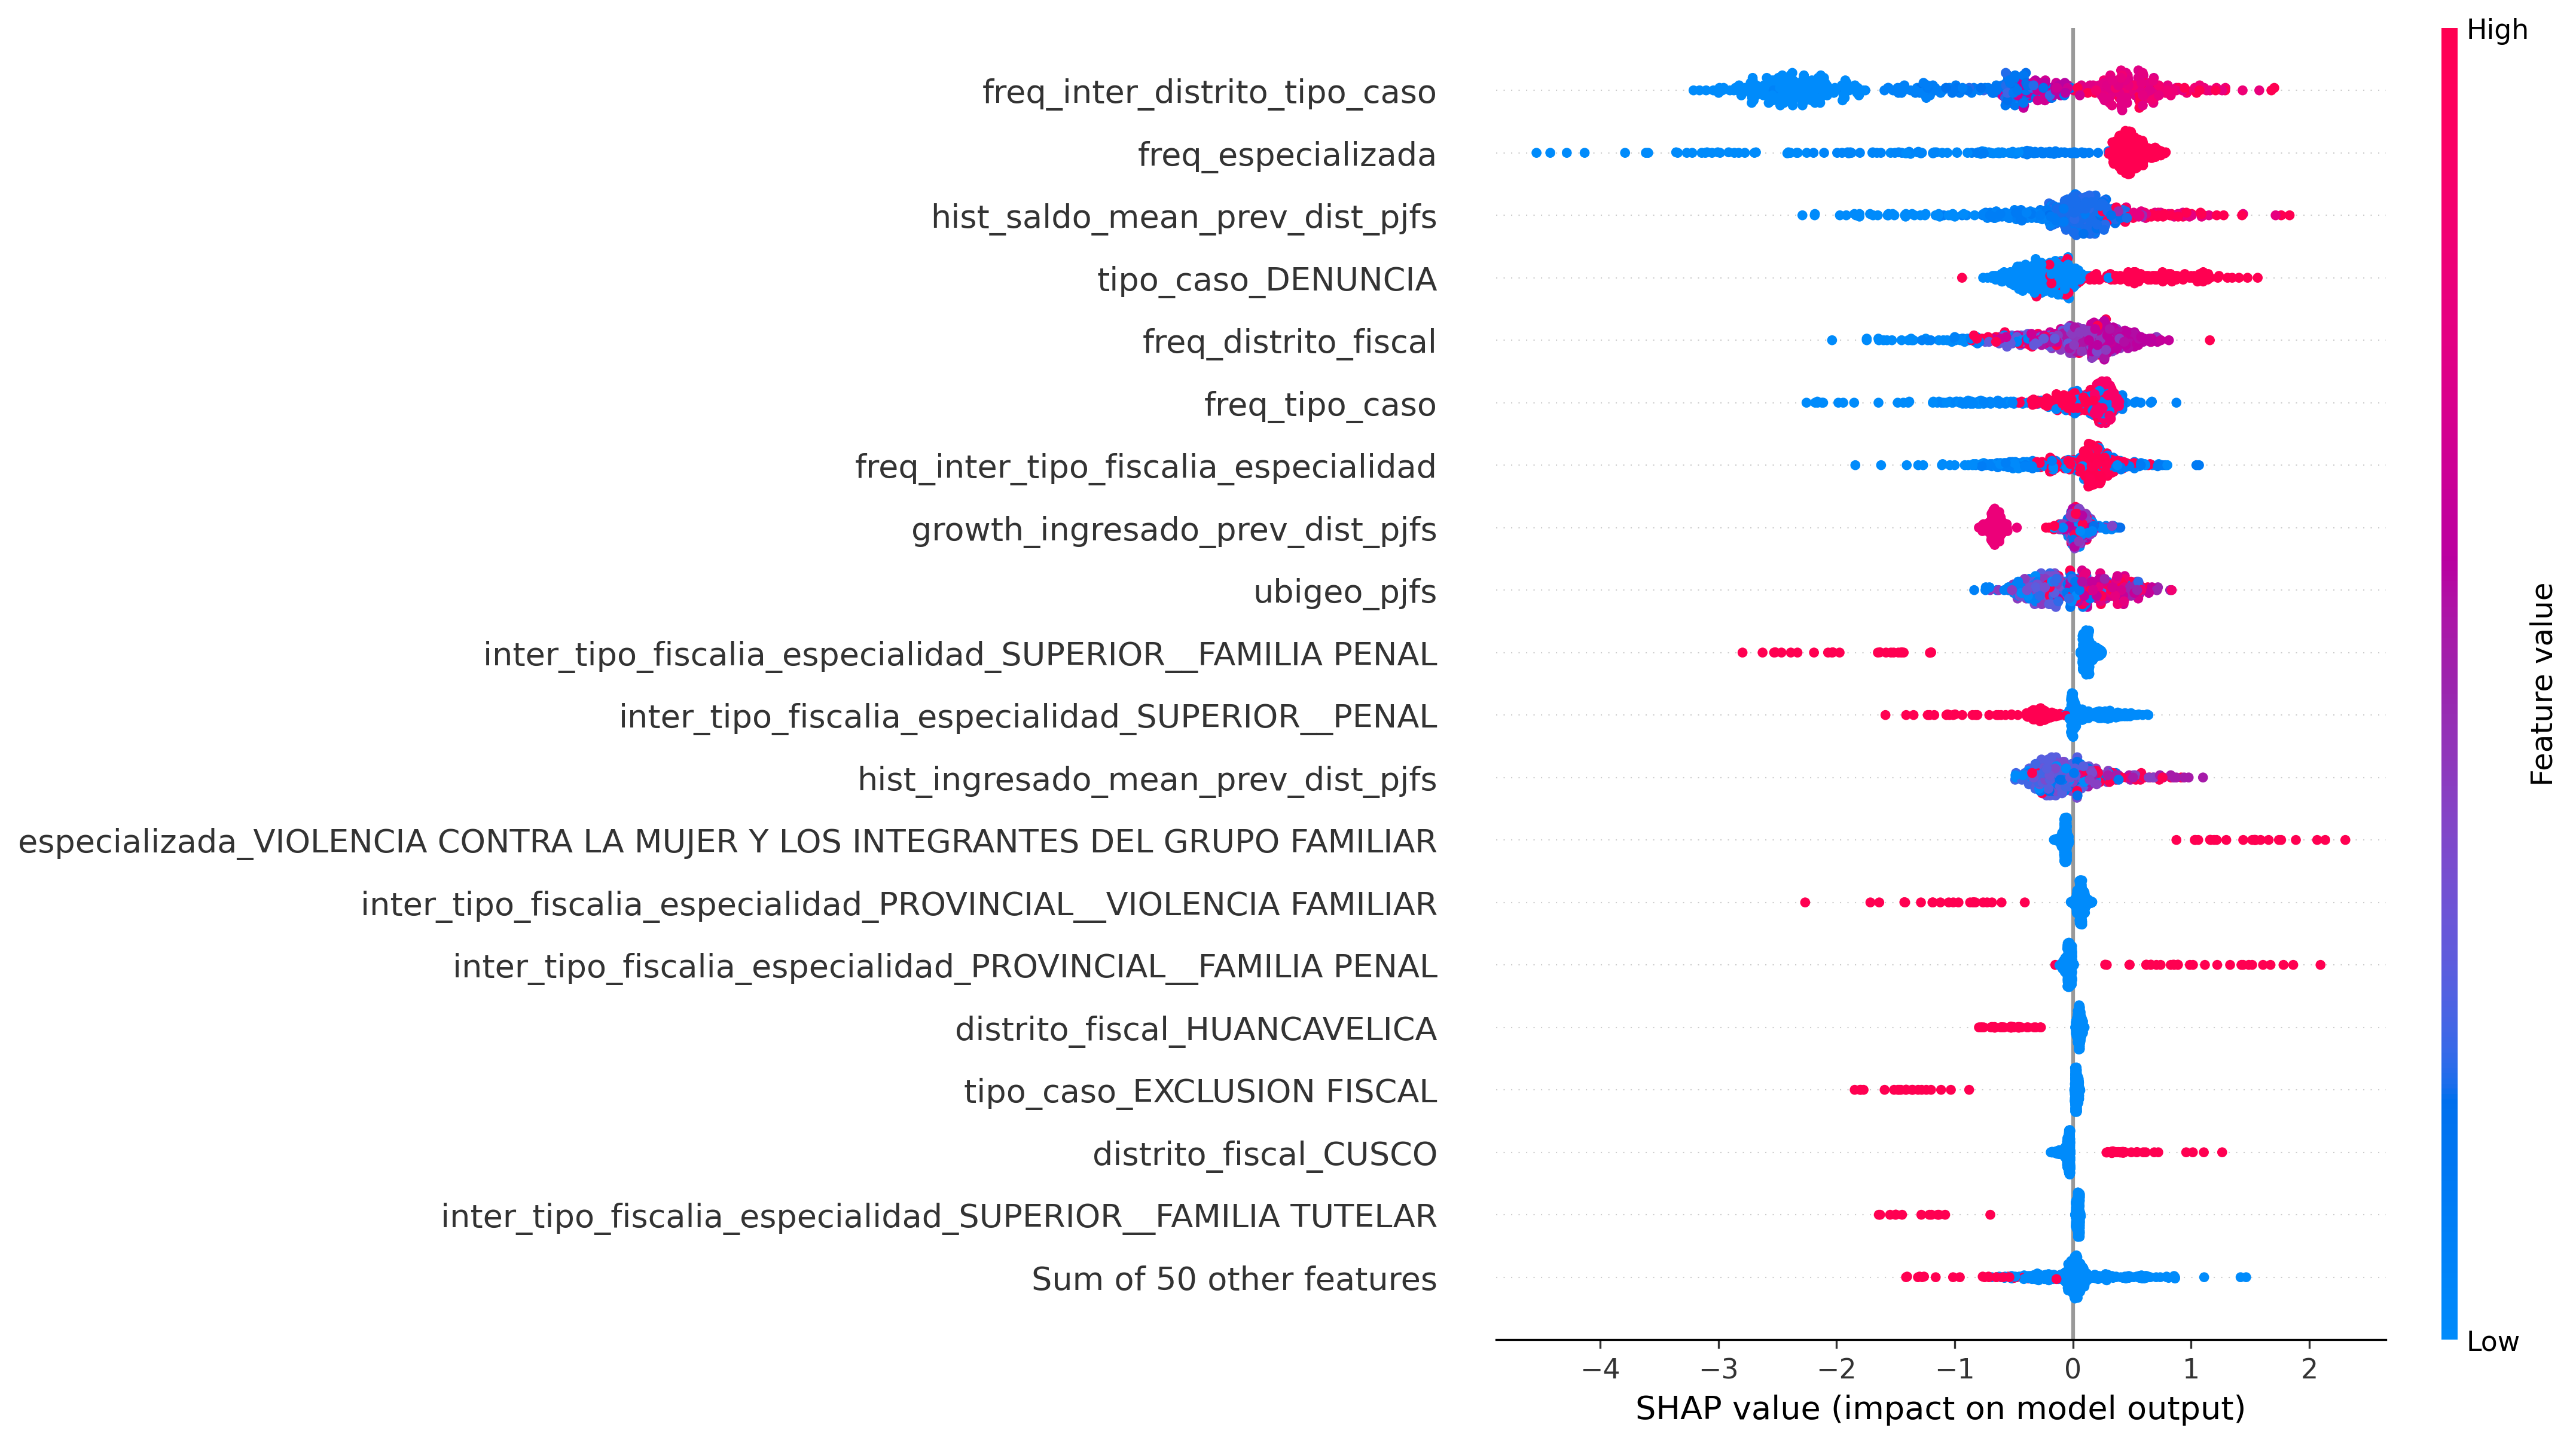
\includegraphics[keepaspectratio]{./media/image10.png}}

\textbf{Figure 10.} SHAP interaction between territorial frequency and
geographic location.

These results suggest that the proxy risk does not depend on geographic
location or case type in isolation, but rather on their specific
combination---consistent with the finding of the ablation study that
removing interaction features degrades predictive performance more than
removing any other individual feature group.

These findings should be interpreted as global predictive associations
learned by the model rather than as causal relationships.

\subsection{B. Operational Impact}\label{b.-operational-impact}

To evaluate the potential operational impact of the model, a sensitivity
analysis based on parametric cost assumptions was conducted for
illustrative purposes only. A 10:1 cost ratio between a false negative
and a false positive was assumed, considering the greater institutional
impact of failing to identify a potential alert.

Under this assumption, a cost of S/ 50,000 was assigned to each false
negative and S/ 5,000 to each false positive. Based on the 2025 test set
(99 FN, 66 FP, 73 TP, and 961 TN), the model yielded an illustrative
estimated loss of S/ 5,280,000 (Table XII). These values do not
represent official costs of the Public Prosecutor\textquotesingle s
Office -- Office of the Attorney General of Peru (MPFN) and are intended
solely to compare operational scenarios.

\textbf{TABLE XII.} OPERATIONAL IMPACT UNDER ILLUSTRATIVE COST
ASSUMPTIONS

{\def\LTcaptype{none} % do not increment counter
\begin{longtable}[]{@{}
  >{\raggedright\arraybackslash}p{(\linewidth - 14\tabcolsep) * \real{0.0909}}
  >{\raggedright\arraybackslash}p{(\linewidth - 14\tabcolsep) * \real{0.0909}}
  >{\raggedright\arraybackslash}p{(\linewidth - 14\tabcolsep) * \real{0.0909}}
  >{\raggedright\arraybackslash}p{(\linewidth - 14\tabcolsep) * \real{0.0909}}
  >{\raggedright\arraybackslash}p{(\linewidth - 14\tabcolsep) * \real{0.1414}}
  >{\raggedright\arraybackslash}p{(\linewidth - 14\tabcolsep) * \real{0.1414}}
  >{\raggedright\arraybackslash}p{(\linewidth - 14\tabcolsep) * \real{0.2121}}
  >{\raggedright\arraybackslash}p{(\linewidth - 14\tabcolsep) * \real{0.1212}}@{}}
\toprule\noalign{}
\endhead
\bottomrule\noalign{}
\endlastfoot
\textbf{FN} & \textbf{FP} & \textbf{TP} & \textbf{TN} & \textbf{FN Cost}
& \textbf{FP Cost} & \textbf{Estimated Loss} & \textbf{FN:FP} \\
99 & 66 & 73 & 961 & S/ 50,000 & S/ 5,000 & S/ 5,280,000 & 10:1 \\
\end{longtable}
}

Note: The reported costs are parametric assumptions (not audited
figures). The causal analysis module (DoubleML-IRM) was designed but not
executed due to technical limitations.

As a future methodological direction, a causal analysis module based on
Double Machine Learning (IRM) was designed; however, it was not executed
because of computational environment limitations. Consequently, its
results are not part of the present study and are proposed as future
work.

In this way, the model predictions provide an objective criterion to
support the preventive prioritization of operational combinations with a
higher proxy risk of prosecutorial congestion, thereby strengthening the
operational planning of the Public Prosecutor\textquotesingle s Office.

These findings are consistent with recent studies identifying
institutional organization and historical operational patterns as
relevant factors for the predictive analysis of judicial systems,
although the present work integrates these elements within a single
reproducible framework
\citep{azaria_alleviating_2024, vasconcelos_analysis_2023}.

\subsection{C. Discussion of Underlying
Mechanisms}\label{c.-discussion-of-underlying-mechanisms}

The dominance of territorial features over historical features is
consistent with the nature of the target. Because it is defined using
percentiles of case backlog and case processing rate, it captures
structural operational overload associated with the installed capacity
of each Prosecutorial District---reflecting heterogeneity across
organizational units---rather than their internal temporal dynamics.
This explains why the ablation study penalizes the removal of
territorial interaction features more severely than the removal of
historical trend features.

The stability of LightGBM relative to CatBoost is consistent with the
latter\textquotesingle s ordered categorical encoding, which is more
sensitive to shifts in category frequencies across years (PSI, Section
III.D.4). Furthermore, DeLong\textquotesingle s test compares
probabilistic ranking performance (ROC-AUC) rather than the
threshold-dependent F1-score; therefore, CatBoost\textquotesingle s
advantage in 2025 reflects a characteristic of that particular temporal
partition rather than a systematic superiority.

The limited contribution of the stacking model is explained by the high
correlation among the base models---four of which are gradient boosting
variants---which reduces the diversity required for a meta-model to
provide additional predictive value.

Finally, the performance of the SVM (F1 = 0.268) confirms the findings
of the unsupervised validation (Section III.C): the decision boundary is
not linearly separable in the feature space, thereby disadvantaging a
linear-margin classifier compared with models capable of capturing
nonlinear interactions.

\section{VI. Limitations}\label{vi.-limitations}

The target variable corresponds to a proxy risk of prosecutorial
congestion constructed using percentile-based rules and does not
constitute an official measure of the Public
Prosecutor\textquotesingle s Office -- Office of the Attorney General of
Peru (MPFN). Although its definition was subjected to sensitivity
analysis, it remains without validation through external expert
judgment. The unit of analysis consists of aggregated combinations of
operational variables rather than individual cases; therefore, the
predictions should be interpreted as support for operational
prioritization rather than for the evaluation of specific cases.

The results were obtained exclusively from data provided by the Public
Prosecutor\textquotesingle s Office of Peru (2019--2026). Although the
framework is reproducible, its application to other judicial systems
requires retraining and recalibration.

The selection of the final model prioritized stability during temporal
validation, even though CatBoost achieved better performance on the 2025
test set, indicating that the relative ranking of models may vary across
consecutive time periods. The economic impact analysis employs
parametric cost assumptions for illustrative purposes only and does not
represent official estimates of the MPFN.

The Double Machine Learning module was designed as a methodological
extension but was not executed because of computational environment
limitations; consequently, the identified relationships correspond
exclusively to predictive associations and should not be interpreted as
causal evidence.

Finally, the limited number of positive observations and the small
sample size of certain subgroups restrict the precision of the fairness
analyses and increase variability across temporal partitions. Therefore,
these results should be interpreted as exploratory evidence.

\section{VII. Conclusions}\label{vii.-conclusions}

This study developed and validated a machine learning framework to
estimate the proxy risk of prosecutorial congestion in the Public
Prosecutor\textquotesingle s Office of Peru, integrating consensus-based
feature selection, multicollinearity auditing, temporal validation, and
model interpretability within a reproducible methodological workflow.
The results demonstrated stable performance on data not used during
training and confirmed the feasibility of the proposed approach for
supporting the early identification of scenarios with higher operational
risk.

The analysis showed that the predictive capability of the model depends
primarily on territorial and institutional patterns, whereas historical
features provide complementary information. The consistency between the
ablation study and the SHAP analysis supports this finding and
demonstrates that the model captures relevant operational configurations
to support the preventive prioritization of operational combinations
with higher estimated proxy risk. Furthermore, the operational impact
analysis demonstrated the potential of the proposed approach to support
planning decisions and the preventive allocation of resources without
replacing the judgment of Public Prosecutor\textquotesingle s Office
practitioners.

From a methodological perspective, the main contribution of this work is
the integration, within a single framework, of robust feature selection,
temporal validation designed to prevent data leakage, robustness
assessment, and model interpretability. This integration helps address a
gap identified in the literature on predictive analytics applied to the
prosecutorial domain, where these components are typically investigated
in isolation.

Future research will focus on validating the definition of the proxy
risk through expert judgment, executing the causal analysis module based
on Double Machine Learning, comparing the operational impact analysis
with official institutional data, extending the temporal training window
as new data become available, and evaluating the transferability of the
framework to other justice systems through retraining and local
validation.


\bibliography{references.bib}



\end{document}
